% Notizen: 
% Irgendwo hin: Da vorher gar keine Entwicklungserfahrung bestand, musste sich erstmal ein klares Bild über die Möglichkeiten geschaffen werden (Eher in den Praxisteil, da es zur Entscheidung gehört)

% Generierung der Bilder mit dem Tool
% Festlegen der Bildgrößen

\section{Konzeption}
% Hier die Entscheidung für Native Apps (Zitat von Apple Human Design Guidelines, und vielleicht generell verschiedene Design ansprechen)

\subsection{Anforderungsanalyse}
Um die Anforderungen an den Prototypen festzulegen und Wünsche sowie Ideen aus dem betrieblichen Umfeld einfließen zu lassen, wurde eine Anforderungsanalyse in Form einer internen Besprechung durchgeführt. Teilnehmer waren Mitarbeiter aus den Abteilungen Marketing und IT. Das Besprechungsprotokoll kann in Abbildung \ref{fig:initial_meeting} eingesehen werden. Auf die in der Besprechung entstandenen Aufgabenpakete wird in den nächsten Kapiteln weiter eingegangen. Im Meeting wurde festgelegt, dass die App parallel für Android und iOS als native Anwendung umgesetzt werden soll. Dies wurde mit Vorerfahrung und dem Wunsch nach einer möglichst angepassten Benutzeroberfläche für alle Plattformen begründet. Außerdem soll die Anwendung Daten zwischenspeichern können, um auch ohne Internet zu funktionieren. Gerade in großen Möbelhäusern kann teils schlechter Mobilfunkempfang herrschen. Im Rahmen dieser Arbeit erfolgte die Umsetzung der Android-App. Außerdem wurde festgelegt, dass sich der Prototyp ausschließlich auf das Smartphone-Format konzentriert. Optimierungen für Tablets können später in Betracht gezogen werden. Für die parallele Entwicklung ist eine intensive Absprache zwischen den beiden Entwicklern nötig. Dafür wurde ein tägliches Meeting angesetzt.

\subsubsection{Schnittstellen}
\label{sec:schnittstellen}
Es werden detaillierte Informationen über alle Modelle und Bezüge benötigt. Dafür sollen Schnittstellen aus anderen Systemen angebunden werden. Im Folgenden werden diese beschrieben. In Abbildung \ref{fig:component_diagram_interfaces} findet sich eine visuelle Darstellung dazu.

\begin{figure}[!htb]
    \centering
    \begin{minipage}[t]{.8\textwidth}
        \caption{Komponentendiagramm Schnittstellen zu anderen Systemen}
        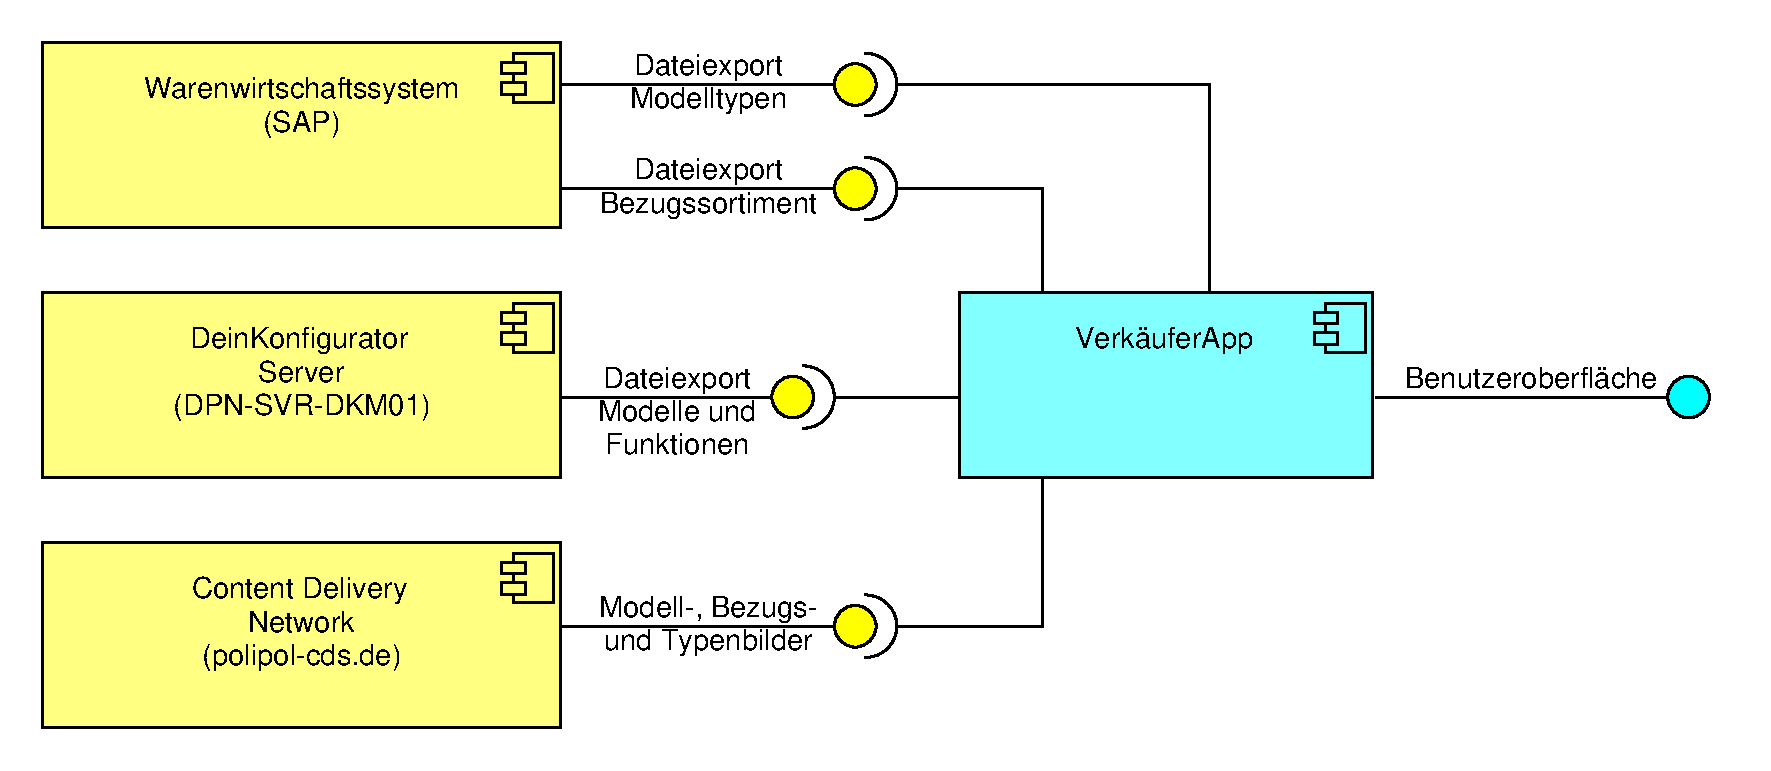
\includegraphics[width=1\textwidth]{img/Komponenten_Schnittstellen.pdf}\\
        \source{eigene Darstellung}
        \label{fig:component_diagram_interfaces}
    \end{minipage}
\end{figure}

In dem \enquote{DeinKonfigurator}-Tool pflegt die Marketingabteilung für jedes Modell Bilder, Eigenschaften und unterstützte Funktionen zu diesen. Die Bilder sind für eine große Anzeige optimiert und finden sich daher überwiegend in einer Auflösung von 1920 x 1080 Pixeln. Zum einen lassen sich Auflösung dieser Größe nicht auf allen Mobilgeräten darstellen, zum anderen verbrauchen hochauflösende Bilder auch mehr Bandbreite bei der Übertragung. Bei schlechten Verbindungen laden die Bilder länger und der Download verbraucht auch große Mengen des Datenvolumens. Daher sollen alle Bilder mit einer automatisierten Routine für Mobilgeräte optimiert werden. Diese Bilder können dann zusätzlich zu den Hochauflösenden über ein bereits eingesetztes \gls{CDN} verteilt werden. Informationen wie Eigenschaften und unterstützte Funktionen können aus der \enquote{DeinKonfigurator}-Datenbank in eine Datei im \gls{JSON}-Format exportiert werden.

Jede Garnitur besteht aus mehreren Typen. Ein Typ ist dabei z. B. eine Rundecke (RE) oder ein Element mit drei Sitzplätzen und einer Armlehne links (3AL). Mehrere Typen lassen sich mit kompatiblen weiteren Typen kombinieren, um eine Zusammenstellung zu bilden. Ein Beispiel für den Typ 3AL und eine Zusammenstellung sind im Anhang auf Seite \pageref{fig:type_plan_example_3al} in den Abbildungen \ref{fig:type_plan_example_3al} und \ref{fig:type_plan_example_combination} zu sehen. Jeder Typ wird im Warenwirtschaftssystem mit einer Beschreibung und seinen Maßen gepflegt. Bilder für die Typen sind über das \gls{CDN} abrufbar. Die Typen sollen ebenfalls in der App zu sehen sein, um dem Verkäufer die verfügbaren Teilelemente eines Modells zur Verfügung zu stellen. Dafür existiert bereits ein Dateiexport im \gls{JSON}-Format der genutzt werden kann.

Zuletzt werden Informationen über alle verfügbaren Bezüge benötigt. Diese liegen ebenfalls im Warenwirtschaftssystem vor und können über vorhandene Schnittstellen in eine \gls{JSON}-Datei exportiert werden. Dazu gehören Stoff- und Lederbezugssortimente. Diese bestehen jeweils aus Bezugsfamilien mit einem Vorschaubild und mehreren Farbvarianten. Jede Variante ist ebenfalls mit einem Bild und einer Bezeichnung versehen. Die Bilder liegen ebenfalls auf dem \gls{CDN} und sollen von dort angebunden werden.

\FloatBarrier
\subsubsection{Funktionale Anforderungen}
\label{sec:funktionale_anforderungen}
% Zentral suche von Garnituren

Die Anforderungen an den Prototypen wurden während der ersten Besprechung in Form von User Stories aufgenommen. Alle Stories für die Android-Entwicklung finden sich in Tabelle \ref{tab:user_stories}.

Die Modellansicht ist ein zentraler Punkt. Ein Verkäufer soll die Möglichkeit haben, sich das gesamte Sortiment nach den Sparten der Polipol-Gruppe anzeigen zu lassen. Auf dieser Übersichtsseite soll jedes Modell mit einem Bild und seinem Namen zu sehen sein, um schnell einen Überblick zu bekommen. Weiterhin wird eine Modellseite benötigt, damit Eigenschaften wie z. B. Stoff- oder Ledergarnitur, Sofa oder Sessel, mögliche Formen und Sitzqualitäten sowie alle kombinierbaren Funktionen eingesehen werden können. Dazu sollen weitere Bilder zu der Garnitur angezeigt werden, um ein visuelles Bild zu ermöglichen. Als Letztes sollen dort alle Typen eines Modells aufgelistet sein, inklusive ihrer Maße. Mit diesen Informationen kann der Verkäufer dem Kunden bereits die Möglichkeiten der Garnitur tiefgehend erklären. Damit der Benutzer die App schnell navigieren kann, wird eine globale Modellsuche nach Namen und ein Modellfilter benötigt. Diese müssen optional in den Sparten eingeschränkt werden können. Weiterhin sollen alle Bezugsfamilien mit ihrem Bezugsfarben angezeigt werden. Auch alle Funktionen der Polipol-Gruppe sollen in der App in einer Liste eingesehen werden können. Zu jeder Funktion, zu der ein Video existiert, soll dieses abgespielt werden können.

\subsubsection{Nicht-funktionale Anforderungen}
Kotlin wurde als Standardprogrammiersprache festgelegt. Diese hat Java abgelöst und wird offiziell von Google empfohlen. Bei schlechter oder fehlender Internetverbindung muss die App funktionieren. Voraussetzung dafür ist lediglich ein einmaliger Start mit aktiver Internetverbindung. Außerdem soll sich die Android-App so weit wie möglich an das Design der Android-Plattform anpassen. Dazu zählt die Einhaltung der Material Guidelines und weitere Plattformeigenheiten. Um die Bilder im \gls{CDN} auf mobile Endgeräte zu optimieren und Daten in der Übertragung einzusparen, wurden verschiedene Auflösungen und Kompressionsalgorithmen getestet. Final wurde festgelegt, dass die Bilder bei gleichem Seitenverhältnis auf die Breite 896 Pixel reduziert im \gls{JPEG}-Format mit einer Qualität von {85\%} automatisch generiert werden sollen.

\FloatBarrier
\subsection{Mockups}
\label{sec:mockups}

\begin{figure}[!htb]
    \centering
    \begin{minipage}[t]{.4\textwidth}
        \caption{Mockup der Sortimentsübersicht}
        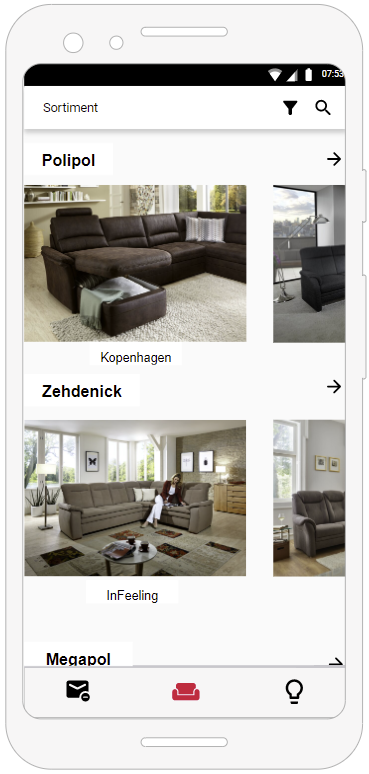
\includegraphics[width=1\textwidth]{img/Mockup_Sortiment.PNG}\\
        \source{eigene Darstellung}
        \label{fig:mockup_sortiment}
    \end{minipage}%
    \
    \begin{minipage}[t]{.4\textwidth}
        \caption{Mockup des Sortimentsfilters}
        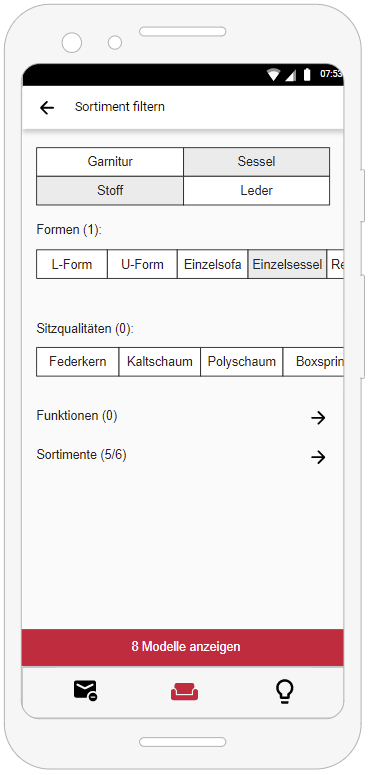
\includegraphics[width=1\textwidth]{img/Mockup_Filter.PNG}\\
        \source{eigene Darstellung}
        \label{fig:mockup_filter}
    \end{minipage}
\end{figure}

Die wichtigsten Seiten der App sollten durch Mockups vor der Umsetzung modelliert werden. In Abbildung \ref{fig:mockup_sortiment} ist die Einstiegsseite in das Modellsortiment zu sehen. Hier sollten, wie in IT-5373 (siehe Tabelle \ref{tab:user_stories}) beschrieben, Modelle nach Sparten gruppiert angezeigt werden. Dies soll durch eine horizontal scrollbare Liste innerhalb einer vertikal scrollbaren Liste ermöglicht werden. Dadurch wird Platz gespart und der Nutzer findet schnell das gewünschte Sortiment. In der Horizontalen sollen jeweils nur die ersten fünf Modelle aus dem Sortiment angezeigt werden, damit es für den Nutzer nicht zu komplex wird. Bei Bedarf kann der Pfeil neben dem Sortimentsnamen angeklickt werden und der Nutzer erhält eine vollständige Übersicht über alle Modelle mit größeren Bildern. Unten befindet sich eine Bottom Navigation Bar um zwischen den zentralen Elementen in der App umzuschalten. Das aktuell markierte Element wird in der Farbe \#d0043b\footnote{Die Farbe wird hier durch eine hexadezimale Farbdefinition bzw. einen \gls{HTML} Farbcode beschrieben} eingefärbt. Dies ist die primäre Farbe aus den Corporate Design Richtlinien der Polipol-Gruppe. Durch die Nutzung einer eigenen Akzentfarbe differenziert sich die App. Am oberen Rand soll eine für Android-Anwendungen typische Toolbar eingebaut werden. Diese enthält jeweils einen Pfeil zur Navigation (falls nicht oberste Seite), einen Namen der aktuellen Seite und weitere Aktionen, die im aktuellen Kontext ausgeführt werden können. In diesem Fall soll von dieser Seite aus der Filter nach Eigenschaften (IT-5379) und die Suche nach Namen (IT-5378) erreichbar sein.

Als zweiter zentraler Punkt gilt die Seite des Sortimentsfilters. Diese ist in Abbildung \ref{fig:mockup_filter} dargestellt. In der App werden die Sparten als \enquote{Sortimente} bezeichnet, da dies für die Verkäufer geläufiger ist. Oben sind die zentralen Eigenschaften platziert. Darunter die Auswahl Sofa oder Sessel und die gewünschte Bezugsart. Die weiteren Eigenschaften sind jeweils gruppiert dargestellt und ermöglichen eine Mehrfachauswahl. Wenn die Anzahl der Möglichkeiten über den Bildschirmrand hinausgeht, kann horizontal gescrollt werden. Durch die Zahl am Gruppennamen ist dem Nutzer immer ersichtlich, ob gerade Elemente aus einer Gruppe ausgewählt sind. Dadurch wird vermieden, dass der Nutzer durch herausgescrollte aktive Elemente in den Ergebnissen unwissentlich eingeschränkt wird. Da die Anzahl der Funktionen zu groß für diese Seite ist, sollen sie auf eine Extraseite ausgelagert werden. Ebenso die Sparten. Die untere rote Schaltfläche ist als zentrales Element gut mit dem Daumen erreichbar. Außerdem wird der Text während des Filterns immer aktuell gehalten. So wird für den Nutzer direkt ersichtlich welche Auswahl die Ergebnisse einschränkt.

% \subsection{Datenquellen und Formate}
% \label{sec:datenquellen_und_formate}
% % Erklärung Tags: Aufteilung Eigenschaften, Formen, Sitzqualitäten, Funktionen

% Die Datengrundlage für die Anwendung bilden die drei Dateiexporte aus Kapitel \ref{sec:schnittstellen}. Die verschiedenen Quellen müssen teilweise über die Modellnummern verknüpft werden.

% Die aus dem DeinKonfigurator-Tool exportierte Datei enthält eine Liste an Funktionen. Beispielhaft wird in Listing \ref{list:json_exmaple_function} die Bettfunktion dargestellt. Jede Funktion besteht aus einem Namen, mehreren Bildern und Videos. Dies ist dafür gedacht in Zukunft mehrere Qualitäten der Bilder bereitzustellen für unterschiedliche Displaygrößen. Daher hat jedes Medium auch eine \enquote{Size}-Eigenschaft. Für die eigentlichen Dateien wird dann mit der \gls{URL}-Eigenschaft auf das \gls{CDN} verwiesen. Diese sollen zur Laufzeit dynamisch geladen werden. Wichtig für die Filterfunktion ist die Angabe einer \enquote{TagReference}. Dies ist eine eindeutige Bezeichnung der Funktion. Dieser Verweis wird auch in der Modelldefinition genutzt um anzuzeigen, dass ein Modell mit dieser Funktion kompatibel ist. Theoretisch handelt es sich bei der Angabe des Verweises um ein Array. In der Praxis ist dies stets ein einzelner Verweis.

% Die Modelldefinitionen befinden sich in der selben exportierten Datei aus dem DeinKonfigurator Tool. Ein Beispiel ist in Listing \ref{list:json_example_model} zu sehen. Ein Modell wird durch seine vierstellige Modellnummer eindeutig identifiziert. Es gibt ein Vorschaubild zu einem Modell. Zusätzlich können weitere Detailbilder angegeben werden. Dabei kann es sich z. B. um Bilder mit Zusammenstellungen oder in Kombination mit einer Funktion handeln. In diesem Fall gibt es ein Bild der Garnitur in einer L-Form. Dies wird ebenfalls über die Eigenschaft \enquote{TagReference} gesteuert. In dem Array \enquote{Tags} befinden sich nun die Verweise die auch in den Funktionsdefinitionen genutzt werden. Darüber können die kompatiblen Funktionen zugeordnet werden. Weitere Eigenschaften die ebenfalls hier angegeben werden sind: der Modelltyp (Garnitur oder Sessel), mögliche Bezugsarten (Stoff oder Leder), Formen (L-Form, U-Form, Einzelsofa, Einzelsessel, Relaxsessel) und verfügbare Sitzqualitäten (Federkern, Kaltschaum, Polyätherschaum und Boxspring). Die Modelldefinition enthält keinen Modellnamen, da es sich hierbei lediglich um kundenunabhängige Daten handelt. Das selbe Modell kann in verschiedenen Möbelhäusern unter unterschiedlichen Bezeichnungen vertrieben werden.

% Die kundenspezifischen Daten müssen aus dem Warenwirtschaftssystem exportiert werden. Der Export der Modelltypen enthält alle Modelle mit ihrer eindeutigen Nummer. Über diese können sie mit denen aus dem DeinKonfigurator-Tool verknüpft werden. Die Modelltypen sind für jeden Kunden individuell. Sie beinhalten dann die kundenspezifischen Modellnamen und die Gruppierung der Modelle nach Sparten. Außerdem werden hier die eigentlichen Typen eines Modells mitgeliefert. Ein Beispiel für ein 3-Sitzer Element mit einer Armlehne an der rechten Seite befindet sich in Listing \ref{list:json_example_type}. Im Attribut \enquote{no} wird die technische Bezeichnung hinterlegt. Diese muss angegeben werden wenn das Möbelhaus diese Garnitur bei Polipol bestellt. Weiterhin werden eine menschenlesbare Beschreibung und eine Bild-\gls{URL} angegeben. Die Maße zu einem Typ werden im Textformat in Zentimeter angegeben. Dies ist nötig, da diese in Fall des 3AL Elementes je nach Variante der Armlehne variieren können.

% Die Bezüge werden ebenfalls aus dem Warenwirtschaftssystem exportiert, da auch diese kundenspezifische Bezeichnungen haben können. Die Bezüge sind in sogenannte Bezugsfamilien unterteilt. Jede Bezugsfamilie entspricht einem Stoff bzw. Leder und ist in mehreren Farben verfügbar. Es gibt jeweils ein Vorschaubild für die Familie und ein Bild für jede einzelne Farbe.

\clearpage

\section{Umsetzung}

\subsection{Projekterstellung}

Um die Entwicklung beginnen zu können, musste zuerst ein neues Projekt mit der Entwicklungsumgebung erstellt werden. Währenddessen wurde festgelegt, dass Android ab der Version 5.0 (\gls{SDK}-Version 21) unterstützt werden soll. Damit kann eine große Nutzergruppe von {94,2\%} angesprochen und gleichzeitig neue Funktionen dieser Version genutzt werden. Unter den Funktionen befinden sich eine bessere Unterstützung für die Material Guidelines, Oberflächenschatten, eine moderne \gls{API} für die Wiedergabe von Videos und die Unterstützung neuerer Kodierungen.\footnote{\cite[Vgl.][]{AndroidFive2021}} Außerdem wurde bereits die benötigte Berechtigung \enquote{android.permission.INTERNET} festgelegt. Damit erhält die App Zugriff auf die Nutzung von Netzwerken. Dies wird für das herunterladen der Bilder benötigt. Die App wurde vorläufig \enquote{PoliSales} genannt. Außerdem wurde von Android Studio eine leere Activity erstellt, welche als Startactivity definiert wurde.

\subsection{Sortimentsseite}
\label{sec:sortimentsseite}
% Alle Sortimente (hier Entwicklung einbauen)
% Alle Sortimente auf einen Blick und die ersten 5 Modelle um mehr visuelles zu bieten
% RecyclerView in RecyclerView (Shared ViewPool)
% Einbau einer Standardsuche über Android ActionView (Freitext, alle Sortimente, QueryHint)

% AssortmentRepo (Datei einbinden)
% Glide ()

Als Erstes sollte die User-Story IT-5373 umgesetzt werden. Diese beinhaltet die Erstellung der Sortimentsseite aus Abbildung \ref{fig:mockup_sortiment}. Für die Listen werden RecyclerViews genutzt. Diese haben die alten ListViews unter Android abgelöst. Eine RecyclerView hat den Vorteil, dass die Elemente innerhalb der Liste beim Scrollen wiederverwendet werden können. Denn Layout-Dateien unter Android stellen nur die Baupläne für die eigentlichen Views dar. Die Erstellung der View, welche dann im Arbeitsspeicher liegt, kann je nach Komplexität des Layouts eine gewisse Zeit und Prozessorressourcen in Anspruch nehmen. Im schlimmsten Fall kommt es durch die dynamische Erzeugung der Views beim Scrollen zu einer spürbaren Verzögerung für den Nutzer. RecyclerViews verwenden deshalb die Views, die aus dem sichtbaren Bereich fallen, an der Stelle, wo eine neue View sichtbar wird wieder.

Für das Laden der Bilder vom \gls{CDN} wurde eine externe Bibliothek verwendet werden. Google empfiehlt dafür \enquote{Glide}. Diese bietet einige Vorteile. Bilder werden z. B. nur in der benötigten Anzeigegröße in den Speicher geladen, um den Arbeitsspeicherbedarf zu reduzieren. Außerdem speichert Glide die Bilder automatisch im Cache der Anwendung zwischen. So sind die Bilder beim nächsten App-Start schneller verfügbar und die mobile Datennutzung wird reduziert. Weiterhin kümmert sich die Bibliothek selber um die Fehlerbehandlung beim Download und erlaubt die Nutzung von Platzhaltern. Mit Platzhaltern kann ein Bild temporär angezeigt werden, bis das Modellbild aus dem \gls{CDN} heruntergeladen wurde. Dadurch, dass der Nutzer visuell erkennt, dass Daten geladen werden, wird die Benutzererfahrung verbessert. Dafür wurden 30 Modellbilder gewählt und manuell, wie in der Abbildung \ref{fig:placeholder} zu sehen, bearbeitet. Bei jeder Bildanfrage wird dann eines dieser Bilder zufällig als Platzhalter gewählt.

\begin{figure}[!htb]
    \centering
    \begin{minipage}[t]{.3\textwidth}
        \caption{Beispiel eines Platzhalters}
        
\includegraphics[width=1\textwidth]{img/Placeholder.jpg}\\
        \source{eigene Darstellung}
        \label{fig:placeholder}
    \end{minipage}
\end{figure}

Für den Prototyp wurde ein Testsortiment aus dem Warenwirtschaftssystem sowie eine Modelldatei aus dem DeinKonfigurator-Tool exportiert. Dieses enthält die meisten Garnituren der Polipol-Gruppe. Die \gls{JSON}-Dateien wurden dann als statische Ressourcen in die App eingefügt. Die Ressourcen können zur Laufzeit über den \enquote{Android Context} abgerufen werden. Der Kontext ist eine Komponente im Android-Umfeld, die den Zugriff auf Anwendungsressourcen und einige Systemschnittstellen regelt. In Listing \ref{list:context_read_raw} ist das Auslesen der Modelldatei gezeigt. Über die Methode \texttt{openRawResource} wird dann ein Datenstrom geöffnet. Dieser wird gelesen und als eine Zeichenkette zurückgegeben. Mithilfe der Bibliothek \enquote{Gson} werden die Daten dann in Kotlin-Objekte umgewandelt. Dies geschieht für alle drei Dateien zum Start der App.

\begin{figure}[!htb]
    \begin{lstlisting}[caption=Auslesen einer Ressource im Textformat über den Android Kontext, label=list:context_read_raw]
context.resources.openRawResource(R.raw.media_classification).bufferedReader().use(BufferedReader::readText)
    \end{lstlisting}
\end{figure}

In Abbildung \ref{fig:screenshot_sortiment} ist das Endergebnis der Sortimentsseite zu sehen. Dabei wurde sich weitestgehend an das Design im Mockup gehalten. Es wurden wenig Farben genutzt und die Größe der Bilder rückt diese in den Vordergrund. Für die einzelnen Modelle wurde die Card-Komponente aus der Material Design Bibliothek genutzt.

\begin{figure}[!htb]
    \centering
    \begin{minipage}[t]{.4\textwidth}
        \caption{Screenshot Sortimentsseite}
        \frame{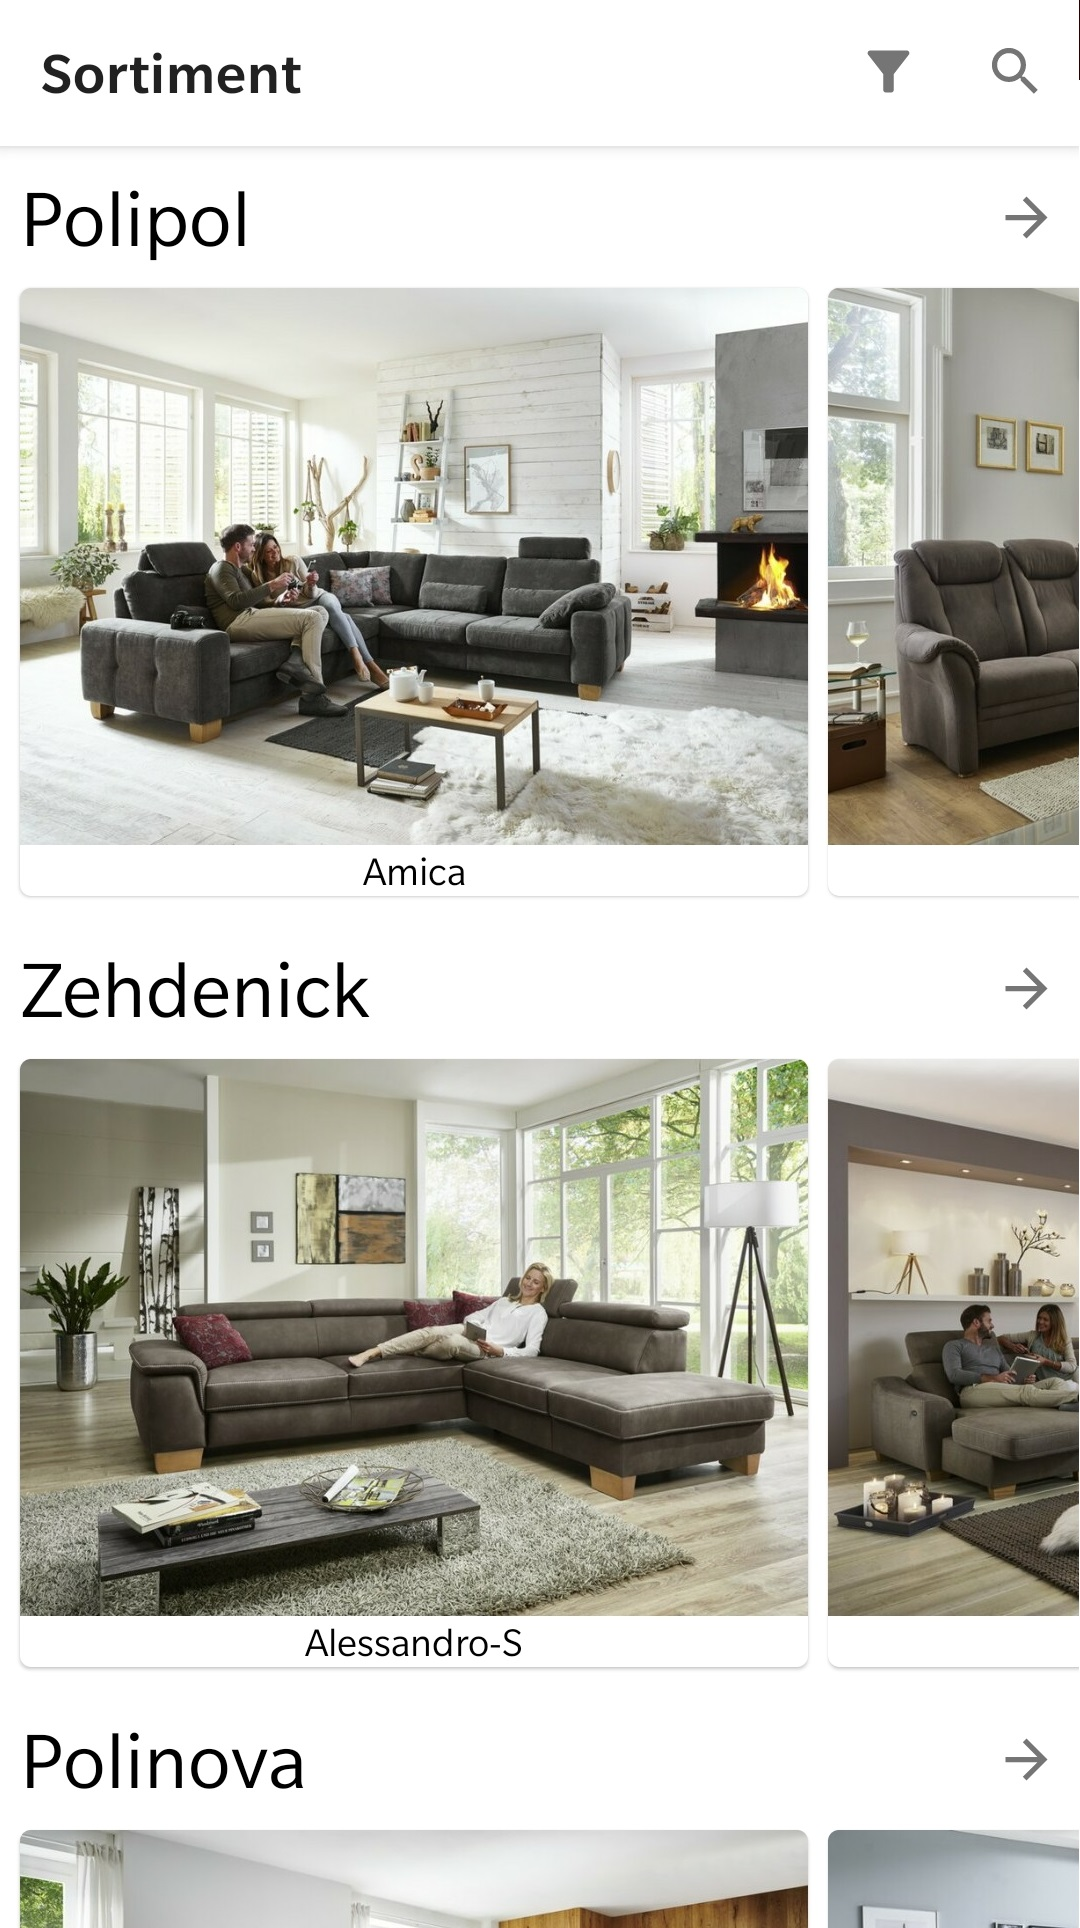
\includegraphics[width=1\textwidth]{img/Screenshot_Sortiment.jpg}}\\
        \source{eigene Darstellung}
        \label{fig:screenshot_sortiment}
    \end{minipage}
\end{figure}

Die Pfeile hinter jeder Sparte zeigen zudem, dass hier noch weiter navigiert werden kann. Dadurch kann der Nutzer alle Modelle zu einer Sparte in einer Liste einsehen. Zwischen den beiden Seite wurde die Navigation mit \enquote{Navigation component} umgesetzt. Dafür mussten beide Seiten in den Navigationsgraphen aufgenommen werden. Dieser wird in einer \gls{XML}-Datei definiert. Die Definition ist in Listing \ref{list:definition_nav_fragments} zu sehen. Von Zeile eins bis sieben ist die Sortimentsübersichtsseite definiert. Bei einer Definition wird jeweils eine Id und das Fragment angegeben. In Zeile vier bis sechs ist eine Navigationsaktion mit einem Ziel definiert. Das Ziel ist in diesem Fall das Fragment für die Modelllistenansicht (\texttt{assortment\_models}). Dadurch werden die beiden Seiten verknüpft. Um Daten mit der Navigation zu übergeben, wurde in Zeile elf das Argument \texttt{AssortmentId} definiert. Darüber wird gesteuert, welche Sparte in dem Fragment angezeigt werden soll. Navigation component generiert automatisch, basierend auf den \gls{XML}-Definitionen, Quellcode, der vom Entwickler zur Navigation verwendet werden kann. Der Navigationsaufruf kann dann über den Code in Listing \ref{list:call_navigate} gestartet werden. Mit der Verknüpfung der beiden Seiten ist die User-Story IT-5373 abgeschlossen.

\begin{figure}[!htb]
    \begin{lstlisting}[caption=Definition der Fragmente für Navigation component, label=list:definition_nav_fragments]
<fragment
    android:id="@+id/assortment_overview"
    android:name="de.polipol.salessupportapp.ui.overview.OverviewFragment">
    <action
        android:id="@+id/actionOpenAssortment"
        app:destination="@id/assortment_models" />
</fragment>
<fragment
    android:id="@+id/assortment_models"
    android:name="de.polipol.salessupportapp.ui.assortmentdetail.AssortmentDetailFragment">
    <argument
        android:name="AssortmentId"
        app:argType="string" />
</fragment>
    \end{lstlisting}
\end{figure}

\begin{figure}[!htb]
    \begin{lstlisting}[caption=Aufruf der Navigation, label=list:call_navigate]
findNavController().navigate(
    OverviewFragmentDirections.actionOpenAssortment(assortment.id)
)
    \end{lstlisting}
\end{figure}

\FloatBarrier
\subsection{Modellseite}
% Modell top bild
% Modell info pdf (für Verkäufer) (Gradle Library!)
% Eigenschaften, Formen, Sitzqualitäten
% Galerie eines Modells (Inspirationen, Aussehen mit Funktionen)
% Typenplan Vorschau (als schnell Überblick) und Absprung

% Informationen zu Eigenschaften:
% Weitere Hilfestellungen für den Verkäufer
% Infos für alles

Als Nächstes wurde die User-Story IT-5374 umgesetzt. Das Ergebnis ist in Abbildung \ref{fig:screenshot_model} zu sehen. Die Tags der Modelle wurden in logische Gruppen, wie schon in Kapitel \ref{sec:funktionale_anforderungen} beschrieben, eingeteilt. Um die Darstellung visuell aufzubereiten, werden hier die Bilder zu den Eigenschaften geladen. Diese sind als statische Ressourcen in der App enthalten und werden über die technischen Bezeichnungen zugeordnet. Wie unter den Funktionen zu erkennen, kann die Liste auch in mehrere Zeilen gebrochen werden. Hier wurde keine horizontal scrollbare Liste gewählt, da dies die Komplexität der Seite steigern würde.

Die User-Story IT-5376 wurde im selben Zug umgesetzt werden. Für die Bildanzeige wurde unten auf der Modellseite eine horizontale RecyclerView eingebaut. Um die Bedienung zu optimieren, wurde ein \texttt{LinearSnapHelper} genutzt. Dieser positioniert das zentral sichtbare Element nach dem Scrollen immer mittig. Die Bilder werden automatisch auf ca. {70\%} der Bildschirmbreite skaliert. So passen sie auf den Bildschirm und erscheinen möglichst groß. Glide übernimmt das Laden der Bilder. Der gesamte Prozess ist in Abbildung \ref{fig:sequence_model} zu sehen. Beim Aufrufen der Seite lädt das ViewModel die Modelldaten asynchron, während für den Nutzer eine Ladeanzeige dargestellt wird. Sobald die Daten verfügbar sind, wird die Seite aufgebaut. Die Eigenschaften können dann eingesehen werden. Nachträglich werden die Galerie Bilder aus den Modelldaten vom \gls{CDN} heruntergeladen und angezeigt.

\begin{figure}[!htb]
    \centering
    \begin{minipage}[t]{0.8\textwidth}
        \caption{Screenshot der Modellseite}
        \frame{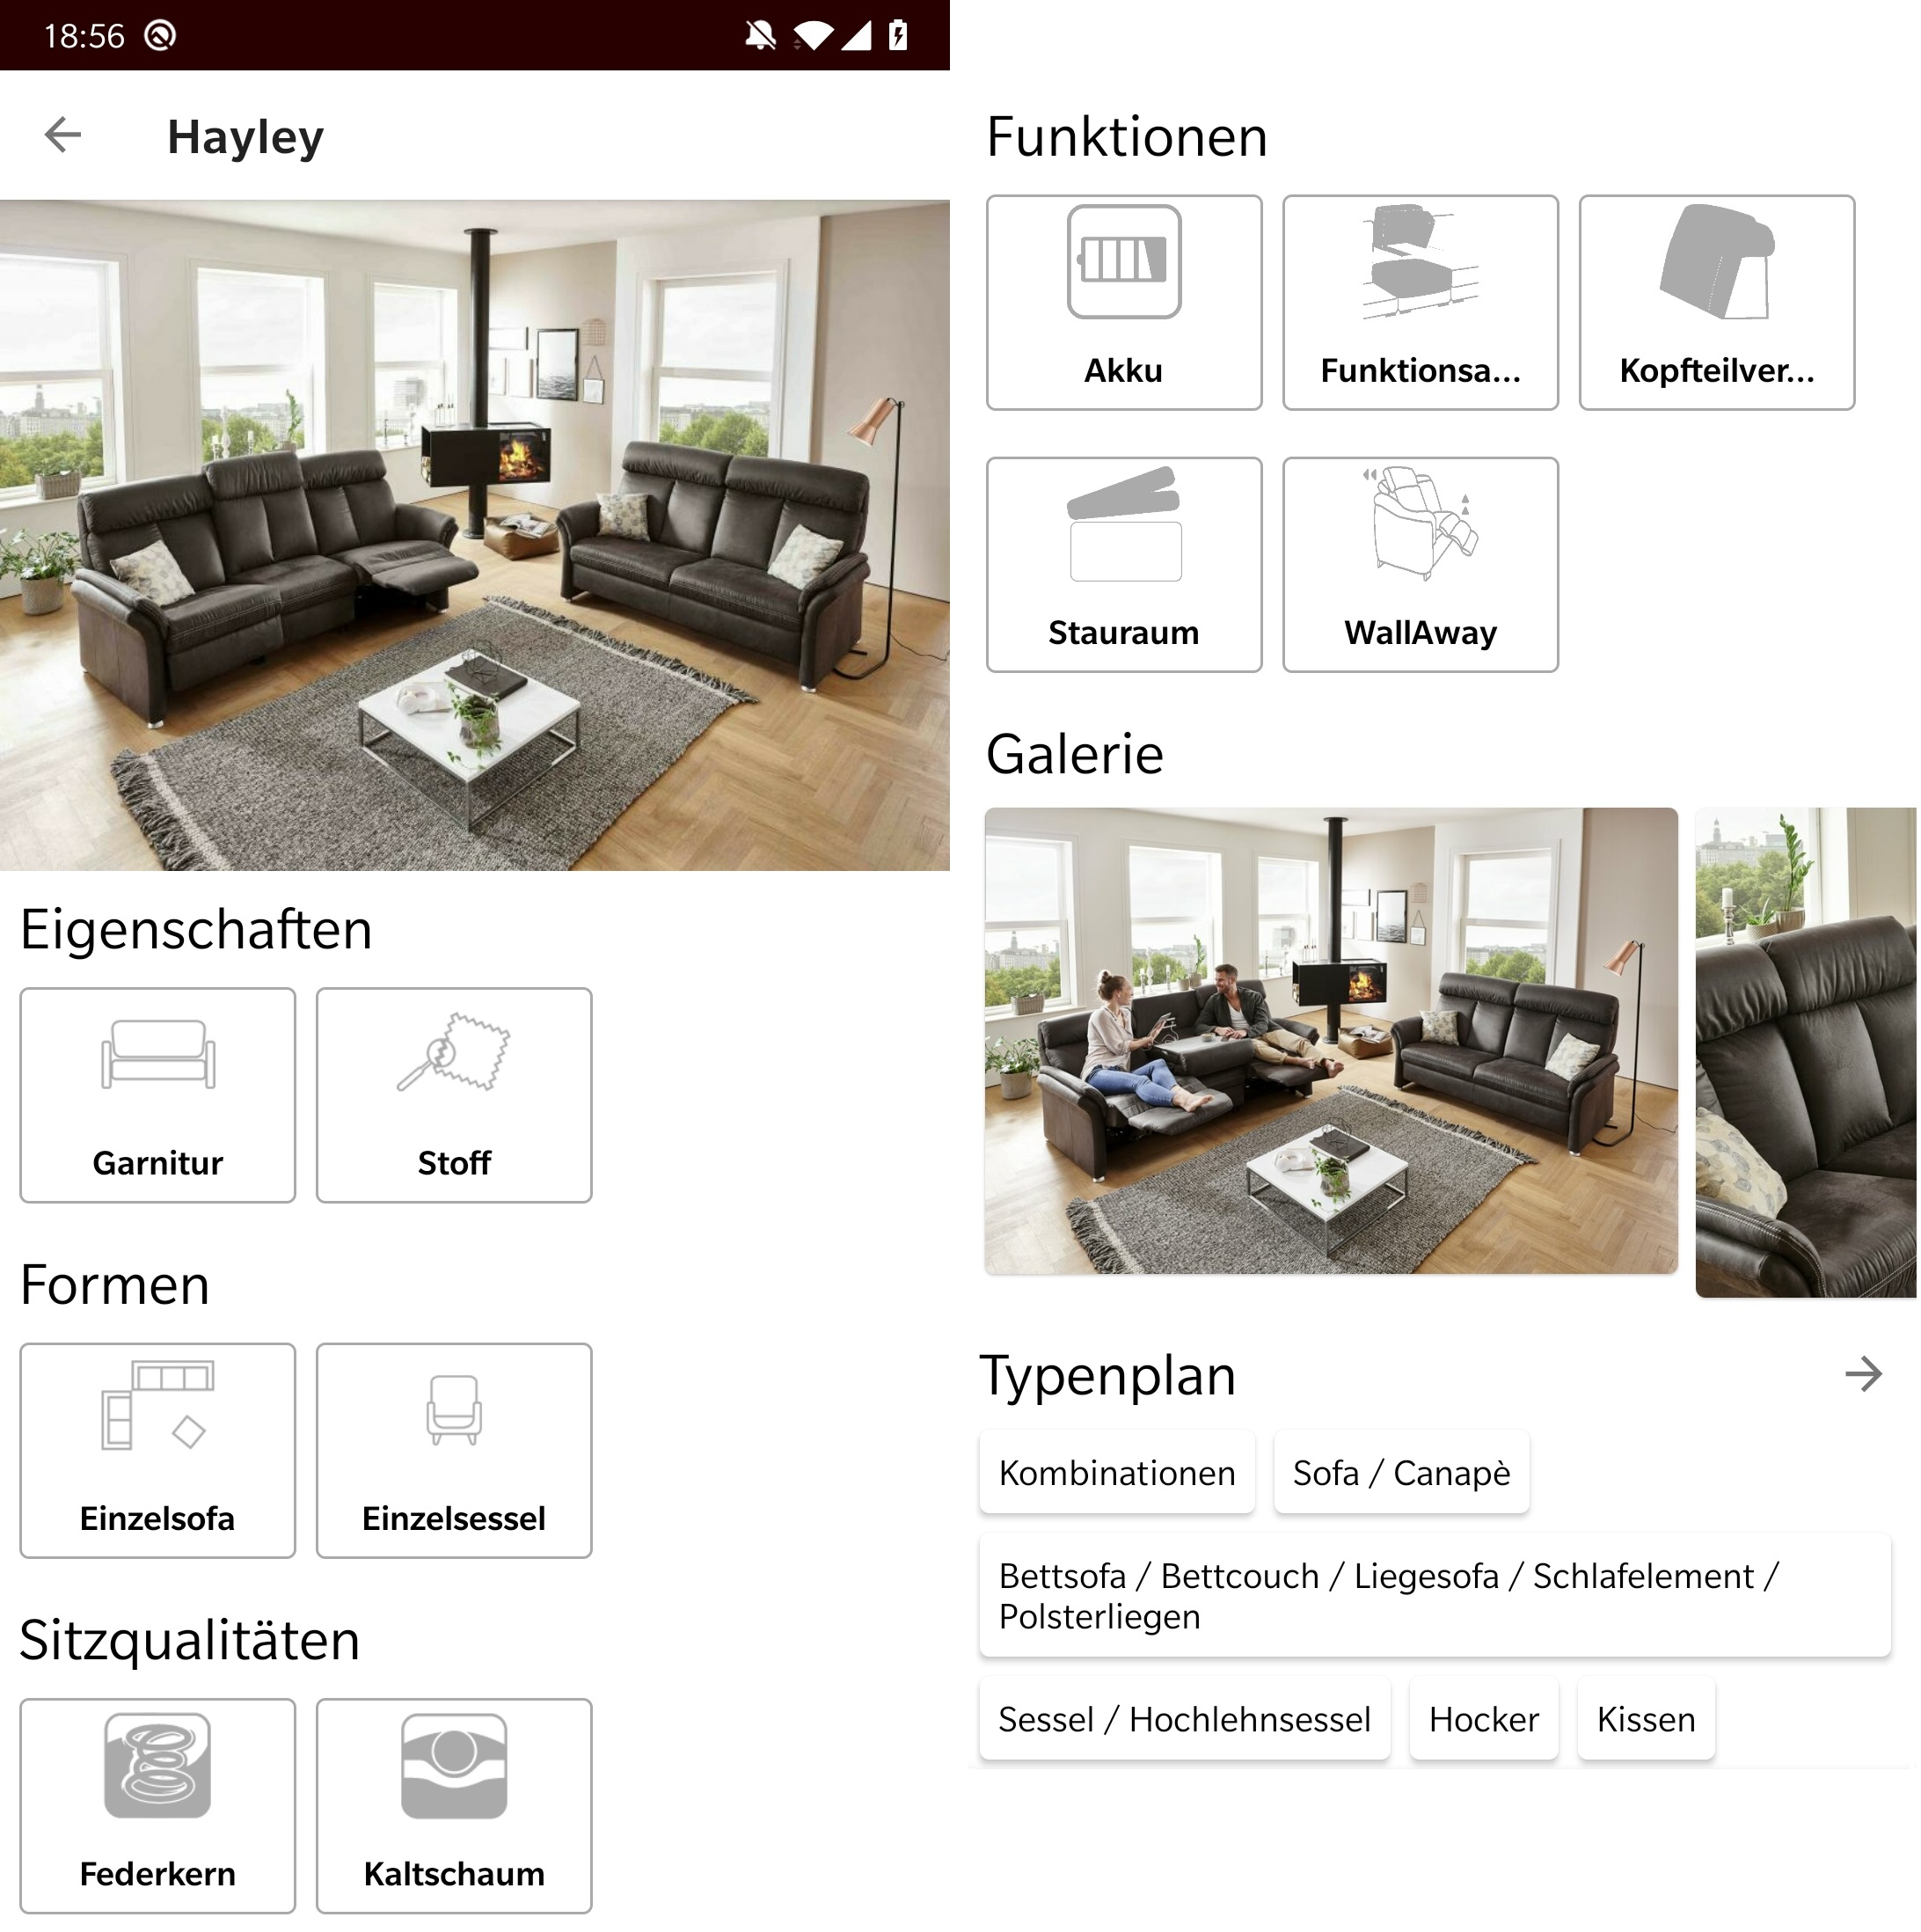
\includegraphics[width=1\textwidth]{img/Screenshot_Model.jpg}}\\
        \source{eigene Darstellung}
        \label{fig:screenshot_model}
    \end{minipage}
\end{figure}

\begin{figure}[!htb]
    \centering
    \begin{minipage}[t]{0.65\textwidth}
        \caption{Sequenzdiagramm zur Modellseite}
        \frame{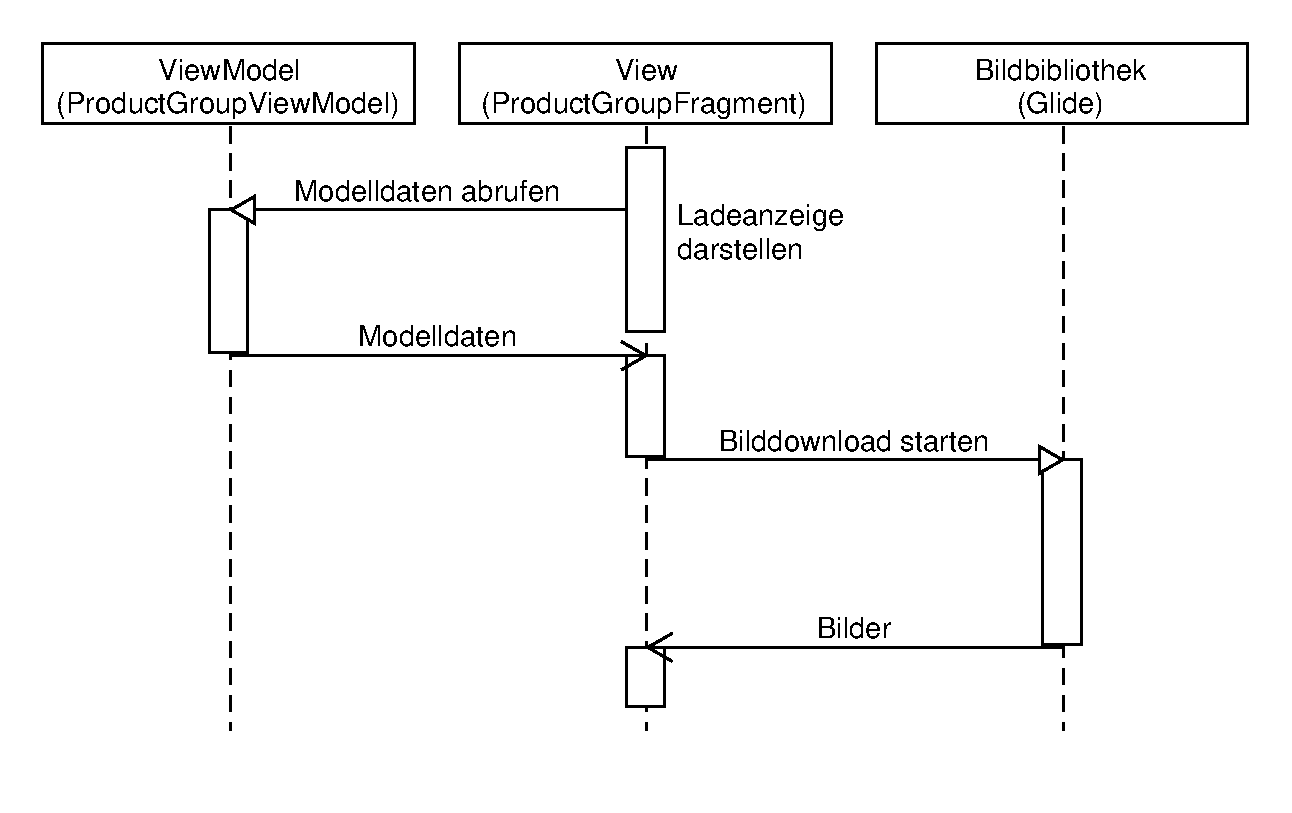
\includegraphics[width=1\textwidth]{img/Sequenzdiagramm_Modellseite_Aufbau.pdf}}\\
        \source{eigene Darstellung}
        \label{fig:sequence_model}
    \end{minipage}
\end{figure}

Um die Modellseite abzuschließen, wurde auch die User Story IT-5375 bearbeitet. Dafür wurden alle Typen gruppiert, wie in Abbildung \ref{fig:screenshot_model}, aufgelistet. Der Nutzer kann über diese Schaltflächen direkt zu den gewünschten Elementen navigieren oder über den Pfeil auf die erste Seite des Typenplans springen. In Abbildung \ref{fig:screenshot_typenplan_uebersicht} ist die eigentliche Typenansicht abgebildet. Da ein Typ meistens in einer rechten und einer linken Ausführung existiert, wurden diese Elemente auf einer Höhe nebeneinander platziert. Die gesamte Ansicht wurde in einem ViewPager implementiert. Dieser erzeugt die Überschriften und ermöglicht das Wechseln zwischen den Gruppen durch horizontales Wischen über den Bildschirm. Als Standardelement aus dem Android \gls{SDK} ist er für Benutzer intuitiv bedienbar. Um insgesamt Platz zu sparen wurde der Beschreibungstext unterhalb der Maßangaben auf jeweils zwei Zeilen begrenzt. Wenn der Text diese Länge überschreitet sind drei Punkte zu erkennen, die auf mehr Content hinweisen. Um den Text vollständig einzusehen, kann der Nutzer die Detailansicht aus Abbildung \ref{fig:screenshot_typenplan_detail} öffnen.

\begin{figure}[!htb]
    \centering
    \begin{minipage}[t]{.4\textwidth}
        \caption{Typenplan: Übersicht}
        \frame{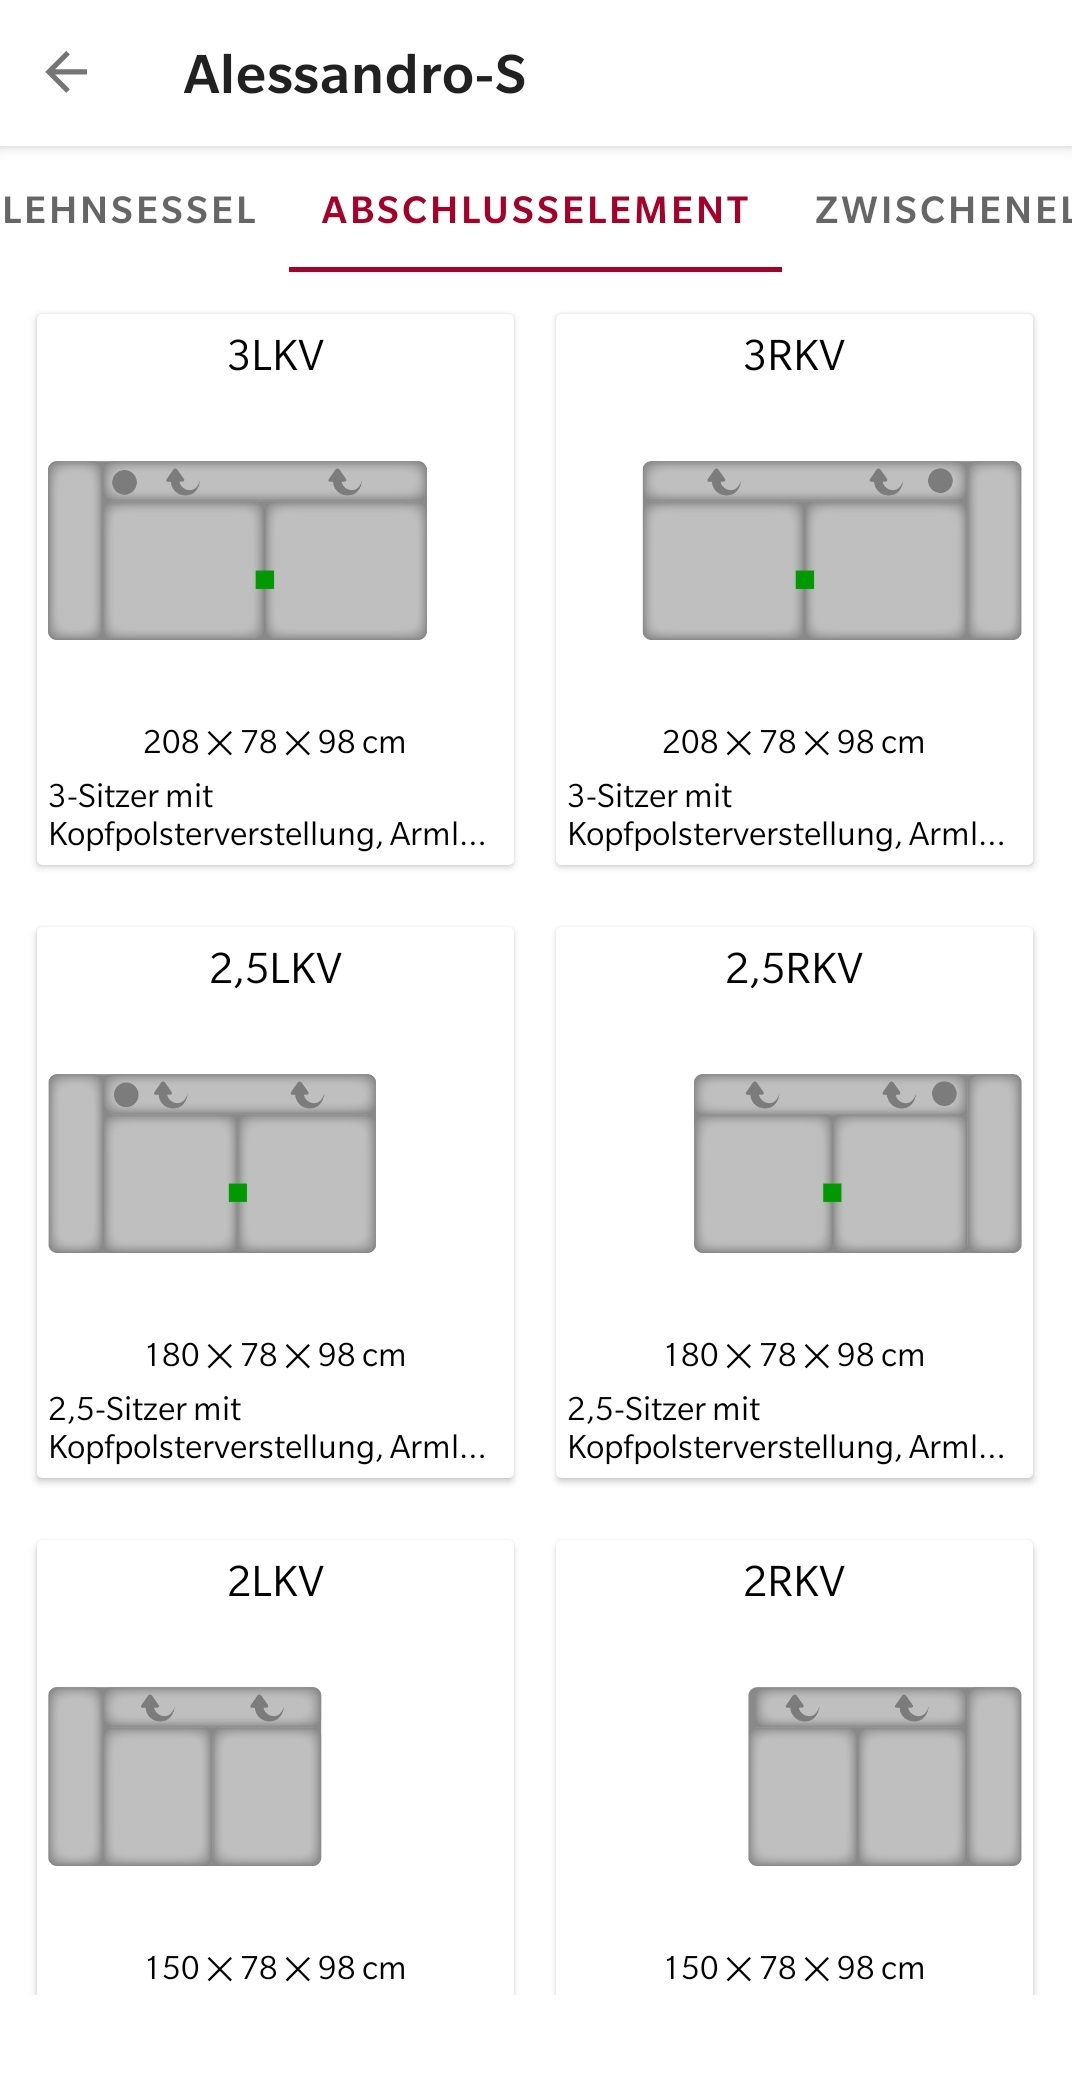
\includegraphics[width=1\textwidth]{img/Screenshot_Typenplan_Uebersicht.jpg}}\\
        \source{eigene Darstellung}
        \label{fig:screenshot_typenplan_uebersicht}
    \end{minipage}%
    \
    \begin{minipage}[t]{.4\textwidth}
        \caption{Typenplan: Detailansicht}
        \frame{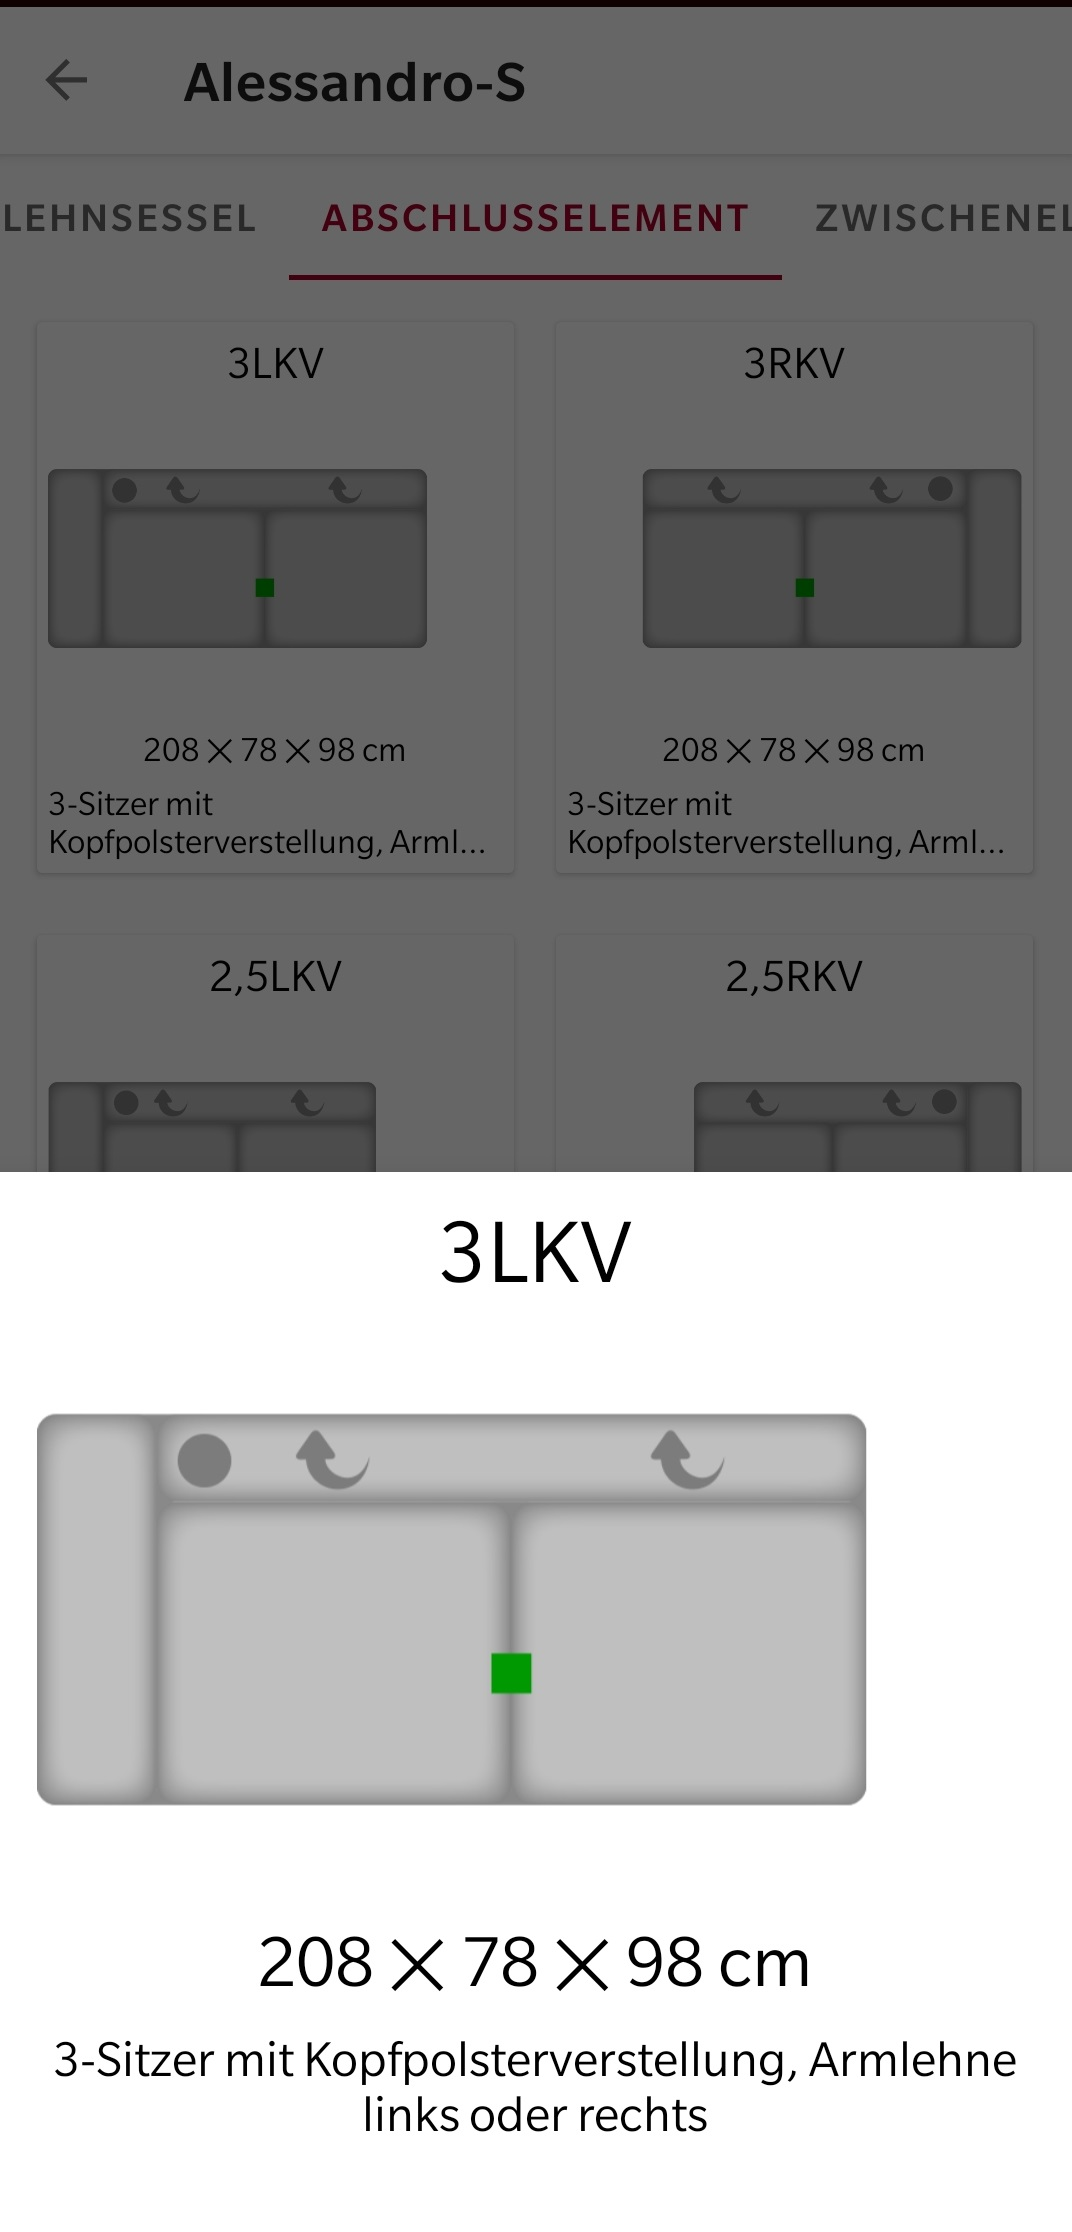
\includegraphics[width=1\textwidth]{img/Screenshot_Typenplan_Detail.jpg}}\\
        \source{eigene Darstellung}
        \label{fig:screenshot_typenplan_detail}
    \end{minipage}
\end{figure}

\FloatBarrier
\subsection{Modellsuche}
Für die Umsetzung der User-Story IT-5378 wurde auf den Seiten der Sortimentsübersicht und der Spartenmodellübersicht jeweils ein Suchsymbol in die Top app bar eingefügt (vgl. Top app bar in Abbildung \ref{fig:screenshot_sortiment}). Je nachdem auf welcher Seite die Suche geöffnet wird, können entweder alle Sparten oder eine Spezifische durchsucht werden. Die Suche erfolgt dann direkt durch Eingabe des Modellnamens in einem Textfeld innerhalb der Top app bar. Die Eingabe wird direkt an ein ViewModel weitergegeben. Dieses führt dann die eigentliche Suche wie in Listing \ref{list:model_search_implementation} zu sehen aus. Um die Anwendung nicht zu blockieren, wird die Suche mit dem Aufruf \texttt{viewModelScope.launch} in einer neuen Koroutine gestartet. Die Ausführung der Koroutinen verwaltet das Android-System. In Zeile vier werden zuerst alle Sortimente (bzw. Sparten) aus dem \texttt{assortimentRepository} Objekt abgefragt. Dann wird in der Zeile fünf die eigentliche Suchmethode \texttt{executeSearch} aufgerufen. Falls der Nutzer die Suche innerhalb einer Sparte geöffnet hat, befindet sich in dem übergebenen Parameter \texttt{assortmentId} die Id der zu durchsuchenden Sparte. Ansonsten ist dieser Wert \texttt{null}. Die zu durchsuchenden Sortimente werden in Zeile 13 gefiltert. In Zeile 14 werden dann alle Modelle (technisch genannt ProductGroups) aus den Sortimenten mit dem Befehl \texttt{flatMap} gesammelt und danach die herausgefiltert, welche den Suchtext im Namen enthalten. Die Suchergebnisse werden dann zurückgegeben und in Zeile sechs in die \texttt{productGroupsLiveData} geschrieben. Das LiveData Objekt ist direkt an die Listenansicht in der View gekoppelt.

\begin{figure}[!htb]
    \begin{lstlisting}[caption=Implementierung der asynchronen Modellsuche, label=list:model_search_implementation]
private fun search(searchText: String){
    viewModelScope.launch {
        try {
            val assortments = assortmentRepository.getAllAssortmentGroups()
            val results = executeSearch(assortmentId, assortments, searchText)
            productGroupsLiveData.postValue(results)
        } catch (ex: Exception) {
            searchExceptionLiveData.postValue(ex)
        }
    }
}
private fun executeSearch(
    assortmentId: String?, assortments: List<Assortment>, searchText: String
): List<ProductGroup> {
    val searchAssortments =
        if (assortmentId.isNullOrEmpty()) assortments else assortments.filter { a -> a.id == assortmentId }
    return searchAssortments.flatMap { a -> a.productGroups }
        .filter { p -> p.name.contains(searchText, true) }
}
    \end{lstlisting}
\end{figure}

\FloatBarrier
\subsection{Sortimentsfilter}
% Re-use der Kacheln (am Beispiel erklären)
% Viel Data Binding
% Prominentes Design des Buttons (Rot, Image Farbe)
% Direktes Feedback
% Extra Seite Sortimente
% Ergebnisse wie Sortimentsansicht

% IT-5379 + IT-5380

Bei der Filterfunktionalität aus der User-Story IT-5379 wurde sich an dem Mockup in der Abbildung \ref{fig:mockup_filter} aus dem Kapitel \ref{sec:mockups} orientiert. Das Ergebnis ist in Abbildung \ref{fig:screenshot_filter} zu sehen. Statt wie auf dem Mockup wurde die Darstellung der Eigenschaften aus der Modellansicht kopiert. Nach der Auswahl einer Eigenschaft aktualisiert sich die Zahl der Modelle auf der unteren Schaltfläche automatisch. So erhält der Nutzer direktes Feedback. Die Funktionsseite ist in Abbildung \ref{fig:screenshot_filter_functions} zu sehen. Um die Benutzererfahrung zu optimieren, wurde die Liste der Funktionen alphabetisch sortiert und jeweils mit Trennbuchstaben versehen. Außerdem kann der Nutzer mit einem Klick auf das Symbol der Mülltonne in der Top app bar seine Funktionsauswahl zurücksetzen. Hinter jeder Funktion ist zudem die Anzahl der Modelle, welche diese unterstützen, zu sehen. Dies hilft dem Nutzer zu erkennen, welche Funktionen die Auswahl stark einschränken können. Dieser Wert aktualisiert sich ebenfalls automatisch mit der Auswahl weiterer Funktionen. Nicht verfügbare Funktionen werden grau hinterlegt und können nicht ausgewählt werden.

\begin{figure}[!htb]
    \centering
    \begin{minipage}[t]{.3\textwidth}
        \caption{Screenshot des Modellfilters}
        \frame{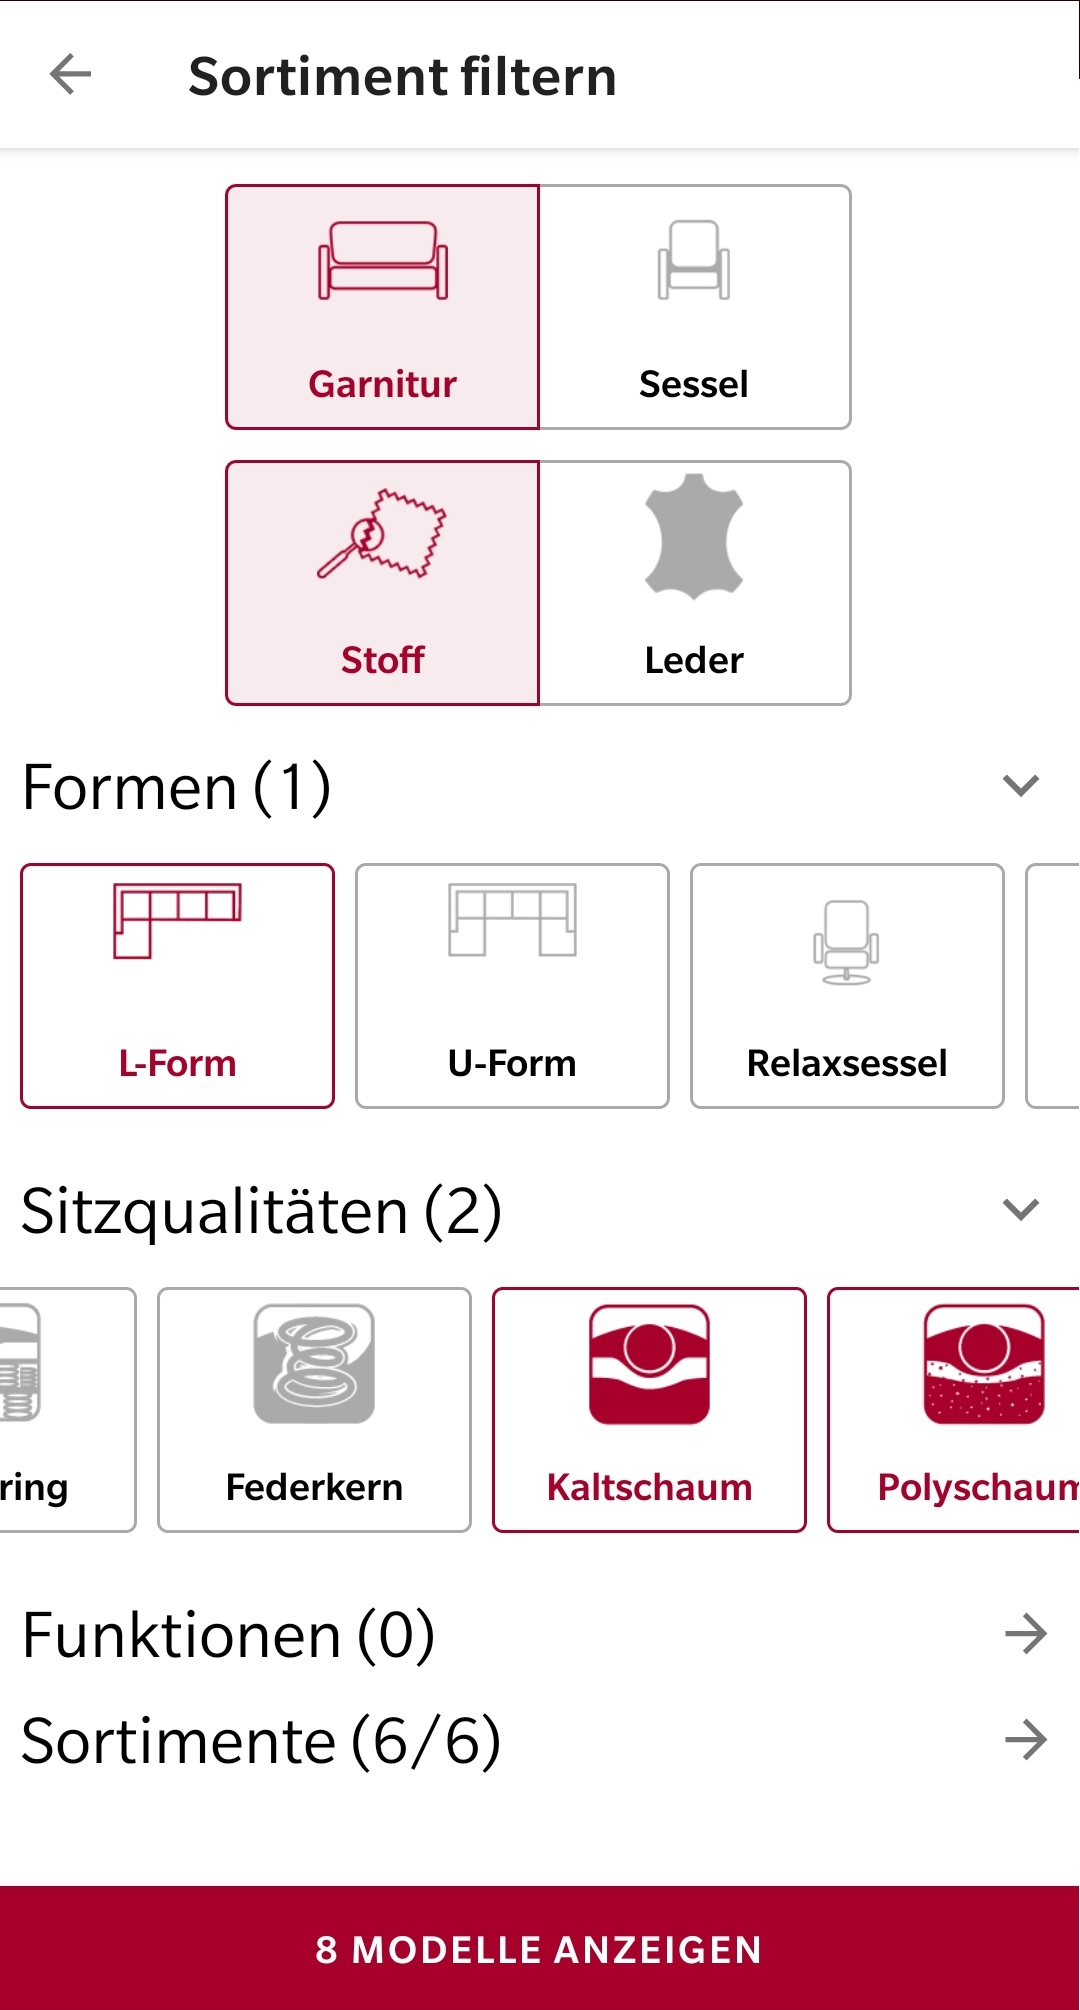
\includegraphics[width=1\textwidth]{img/Screenshot_Filter.jpg}}\\
        \source{eigene Darstellung}
        \label{fig:screenshot_filter}
    \end{minipage}%
    \
    \begin{minipage}[t]{.3\textwidth}
        \caption{Screenshot der Funktionsauswahl}
        \frame{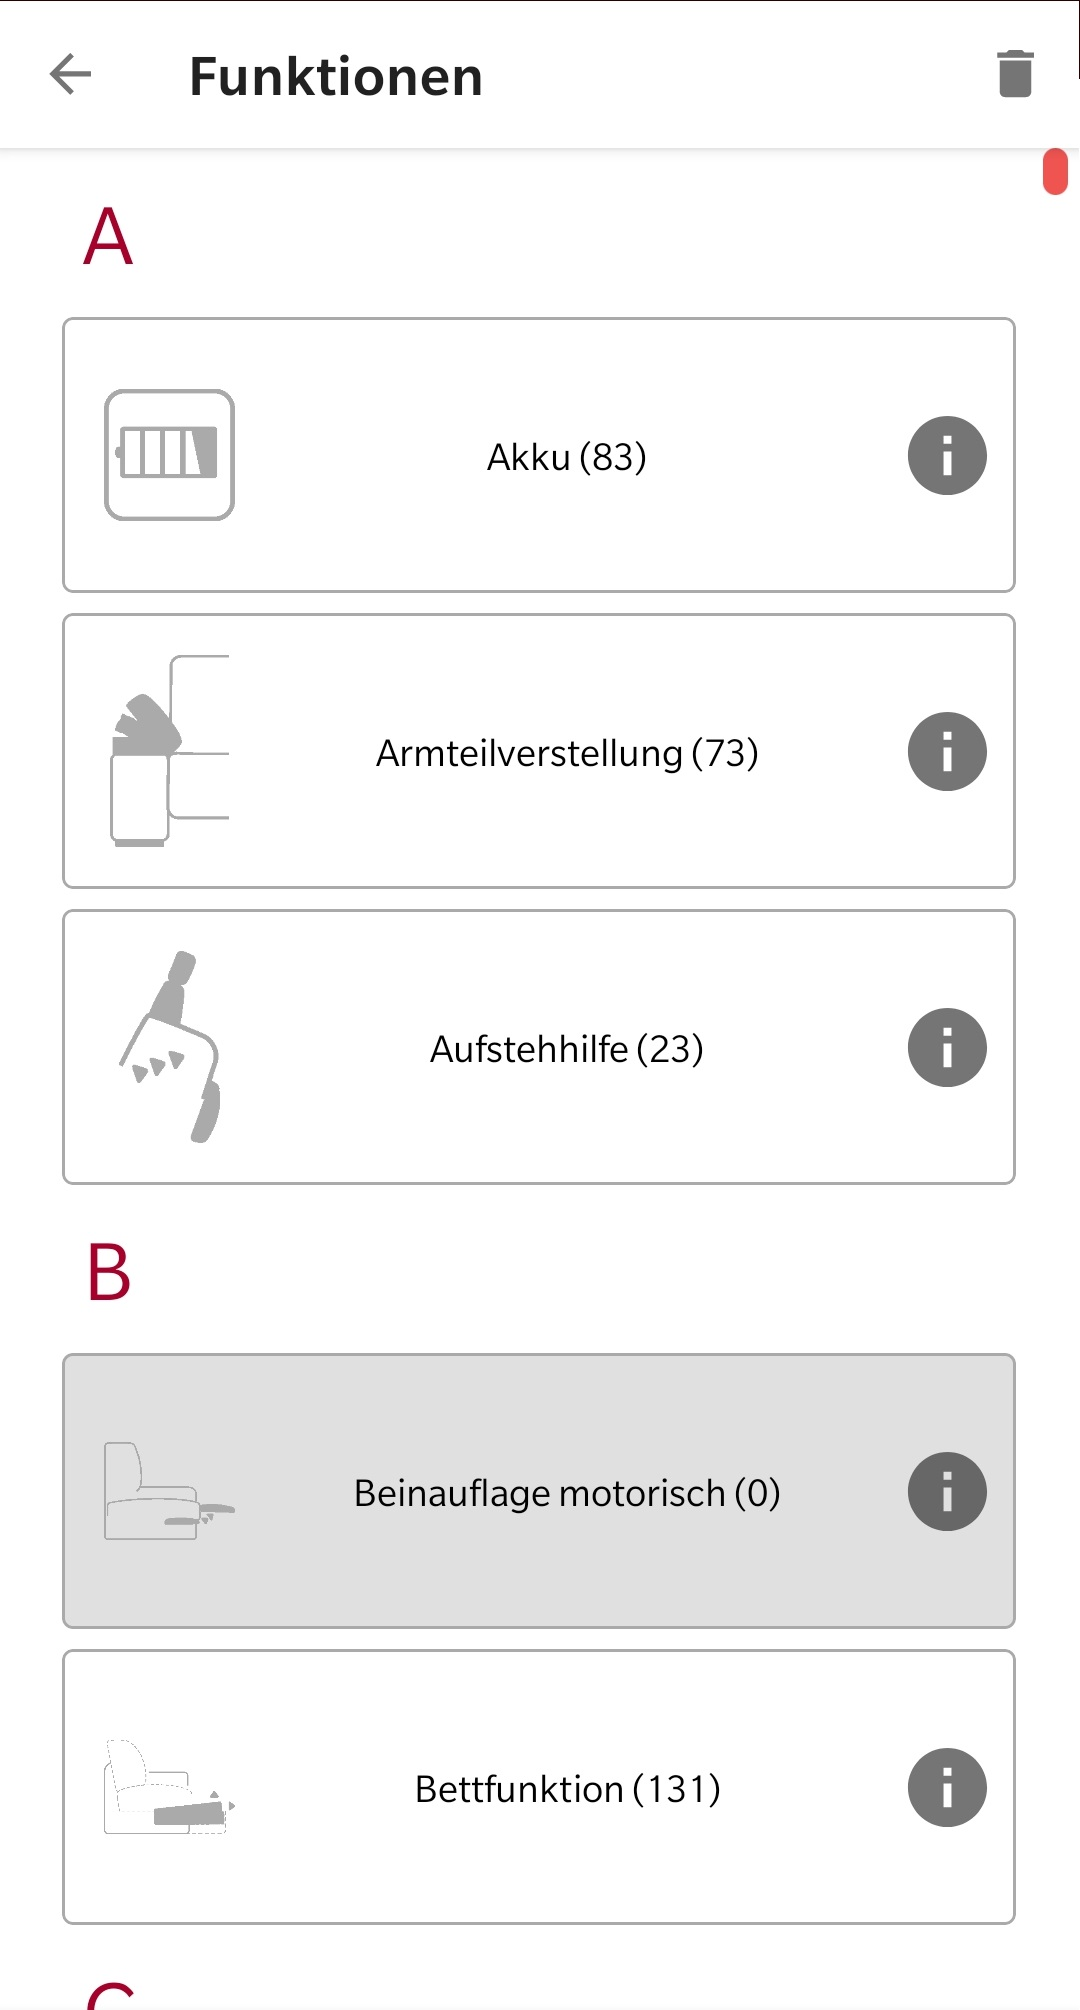
\includegraphics[width=1\textwidth]{img/Screenshot_Filter_Funktionen.jpg}}\\
        \source{eigene Darstellung}
        \label{fig:screenshot_filter_functions}
    \end{minipage}%
\end{figure}

Im selben Zug wurde auch die User-Story IT-5380 umgesetzt. Dafür wurde die Filterfunktion zusätzlich um die Einschränkung der Sparten erweitert. Dies wurde durch den in Abbildung \ref{fig:screenshot_filter} zu erkennenden Abschnitt \enquote{Sortimente} umgesetzt. In diesem kann ähnlich wie bei den Funktionen in einer Unterseite die Auswahl der Sparten eingeschränkt werden.

\FloatBarrier
\subsection{Funktionsseite}
\label{sec:funktionen}
% Alle Funktionen mit Icon
% Alphabetisch getrennt, schneller finden (Denn man sucht meistens nach Namen, hier kein Bild wie bei Modelle)
% Video zu Funktionen
% Möglichkeit in Filter (Wiederverwendung der Ergebnisseite)
% Eventuell sagen das es nicht beendet wurde (Crash bei Klick auf Filterbutton)

% IT-5381

Für die Umsetzung der Story IT-5381, der Einbindung einer Funktionsliste mit ggf. Videos, wurde die Navigation innerhalb der App erweitert. Dafür wurde eine Bottom Navigation Bar benutzt. Die aktuelle Sortimentsübersichtsseite aus dem Kapitel \ref{sec:sortimentsseite} wurde unter den Punkt Sortiment gesetzt. Neu hinzugefügt wurden die Punkte Neuigkeiten und Wissen. Der Punkt Neuigkeiten wird später implementiert.

\begin{figure}[!htb]
    \centering
    \begin{minipage}[t]{0.4\textwidth}
        \caption{Darstellung der unteren Navigationsleiste}
        \frame{
\includegraphics[width=1\textwidth]{img/Screenshot_Bottom_Nav.jpg}}\\
        \source{eigene Darstellung}
        \label{fig:screenshot_bottom_nav}
    \end{minipage}
\end{figure}

% Aus der Filteransicht konnte die Listenansicht der Funktionen hier übernommen werden. Lediglich die Informationsschaltfläche auf der rechten Seite wurde durch einen Pfeil ausgetauscht (siehe Abbildung \ref{fig:screenshot_knowledge_functions}).

\begin{figure}[!htb]
    \centering
    \begin{minipage}[t]{0.4\textwidth}
        \caption{Darstellung einer Funktion}
        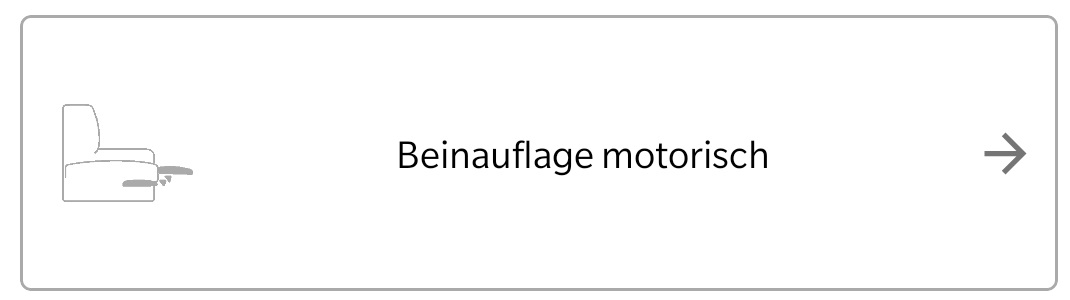
\includegraphics[width=1\textwidth]{img/Screenshot_Knowledge_Function.jpg}\\
        \source{eigene Darstellung}
        \label{fig:screenshot_knowledge_functions}
    \end{minipage}
\end{figure}

Die Funktionsseite, wie in Abbildung \ref{fig:screenshot_knowledge_function_page} zu sehen, enthält eine Kurzbeschreibung und ein Video. Dieses zeigt jeweils die Bedienung und Nutzung der Funktion. Das Video wurde mithilfe der von Google entwickelten Bibliothek \enquote{ExoPlayer} eingebunden. Diese bietet eine flexible Alternative zur Android MediaPlayer \gls{API} und vereinfacht das Abspielen von Videos unter allen Android Versionen bis 4.1 (\gls{SDK}-Version 16). Trotzdem müssen in diesem Fall einige Unterschiede zwischen den Android-Versionen beachtet werden. In Listing \ref{list:exoplayer_lifecycle} ist der Quellcode für die Verwaltung des ExoPlayers zu sehen. Die Methode \texttt{initializePlayer} erzeugt die ExoPlayer Instanz und übergibt die Video \gls{URL}. Damit fragt der ExoPlayer auch die nötigen Ressourcen zum Dekodieren und Anzeigen des Videos beim Android-System an. Die Methode \texttt{releasePlayer} gibt diese Ressourcen wieder frei. Ohne diesen Aufruf kann es zu Speicherlecks kommen. Über die Eigenschaft \texttt{Util.SDK\_INT} wird die aktuell ausgeführte Android \gls{SDK}-Version abgefragt. Jede Activity und jedes Fragment besitzt die vier gezeigten Methoden. Diese können bei Bedarf überschrieben werden. \texttt{onStart} wird vom System aufgerufen, sobald die View für den Nutzer sichtbar wird. \texttt{onResume} sobald der Nutzer mit ihr interagieren kann. \texttt{onPause} wird dann aufgerufen, wenn sich die View nicht länger im Vordergrund befindet. Und \texttt{onStop} sobald die View nicht mehr sichtbar ist. Eine View kann sichtbar aber nicht im Vordergrund sein, wenn sich z. B. ein Dialogfenster über dieser befindet. Seit der Android Version 7.0 (\gls{SDK}-Version 24) wird der Multi-Window-Modus unterstützt. Damit können zwei Apps parallel nebeneinander auf dem Bildschirm geöffnet sein. In einem solchen Fall kann sich die App ebenfalls in einem sichtbaren, aber inaktiven Zustand befinden. Um zu vermeiden, dass die Medienwiedergabe abbricht, wenn der Nutzer mit der zweiten App interagiert, darf der MediaPlayer erst in der \texttt{onStop} Methode die Ressourcen freigeben. Ebenso muss der MediaPlayer schon in der \texttt{onStart} Methode initialisiert werden. Problematisch ist allerdings, dass Android unter der Version 7.0 (unter \gls{SDK}-Version 24) die benötigten Ressourcen nur an sichtbare und aktive Views vergibt. Um diese Problematik zu umgehen muss im Quellcode die Version abgefragt und korrekt gehandelt werden.

\begin{figure}[!htb]
    \centering
    \begin{minipage}[t]{0.4\textwidth}
        \caption{Screenshot der Funktionsseite}
        \frame{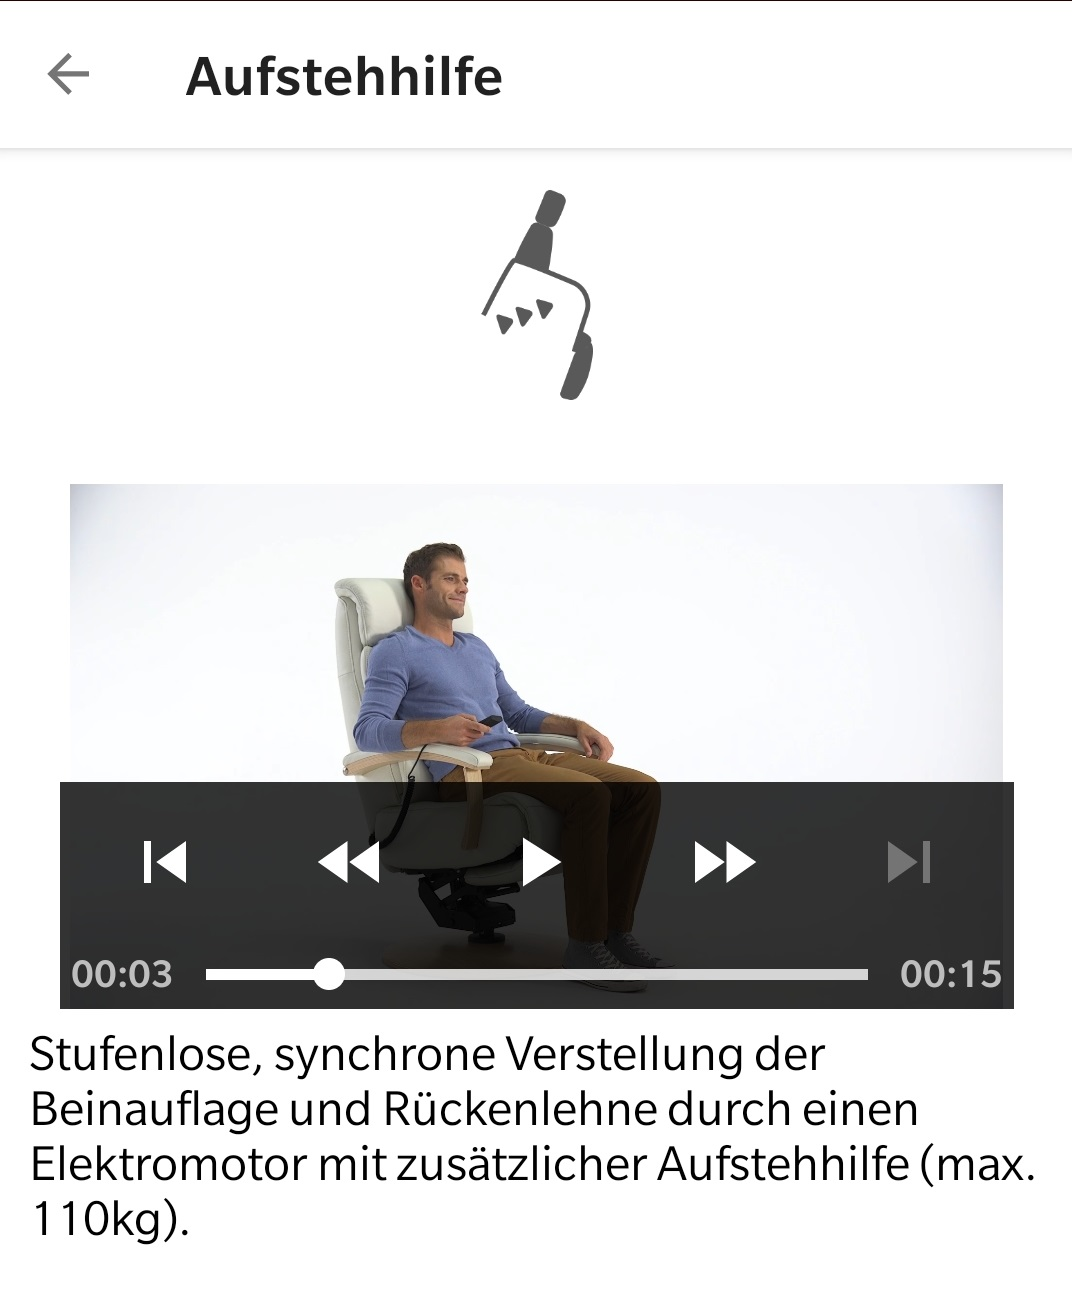
\includegraphics[width=1\textwidth]{img/Screenshot_Function_Page.jpg}}\\
        \source{eigene Darstellung}
        \label{fig:screenshot_knowledge_function_page}
    \end{minipage}
\end{figure}

\begin{figure}[bht]
    \begin{lstlisting}[caption=Verwaltung der ExoPlayer Ressourcen, label=list:exoplayer_lifecycle]
override fun onStart() {
    if (Util.SDK_INT >= 24) initializePlayer()
}
override fun onResume() {
    if (Util.SDK_INT < 24) initializePlayer()
}
override fun onPause() {
    if (Util.SDK_INT < 24) releasePlayer()
}
override fun onStop() {
    if (Util.SDK_INT >= 24) releasePlayer()
}
    \end{lstlisting}
\end{figure}

\FloatBarrier
\subsection{Bezugsseite}
% ViewPager mit CustomView (Implementierung zeigen)
% Vorschau wie bei Modellen

% IT-5382 + IT-5383

Als Nächstes sollten auch die Bezüge in die App eingebaut werden. Die Seite einer Bezugsfamilie (siehe Abbildung \ref{fig:screenshot_cover_family}) besteht aus einem ViewPager mit dem alle Farben zu einem Stoff eingesehen werden können und einem TabLayout am unteren Rand. Mit diesem können die Farben schneller durchsucht werden. Die beiden Elemente sind miteinander verknüpft. Wenn eine Farbe im TabLayout ausgewählt wird, scrollt der ViewPager auch diese Farbe in die Ansicht. Wenn im oberen ViewPager gescrollt wird, bewegt sich auch die Ansicht des TabLayout mit. Dies geschieht durch die Komponente TabLayoutMediator aus der AndroidX Bibliothek. Damit sind auch die User-Stories IT-5382 und IT-5383 erledigt.

\begin{figure}[!htb]
    \centering
    \begin{minipage}[t]{.4\textwidth}
        \caption{Seite der Bezugsfamilie}
        \frame{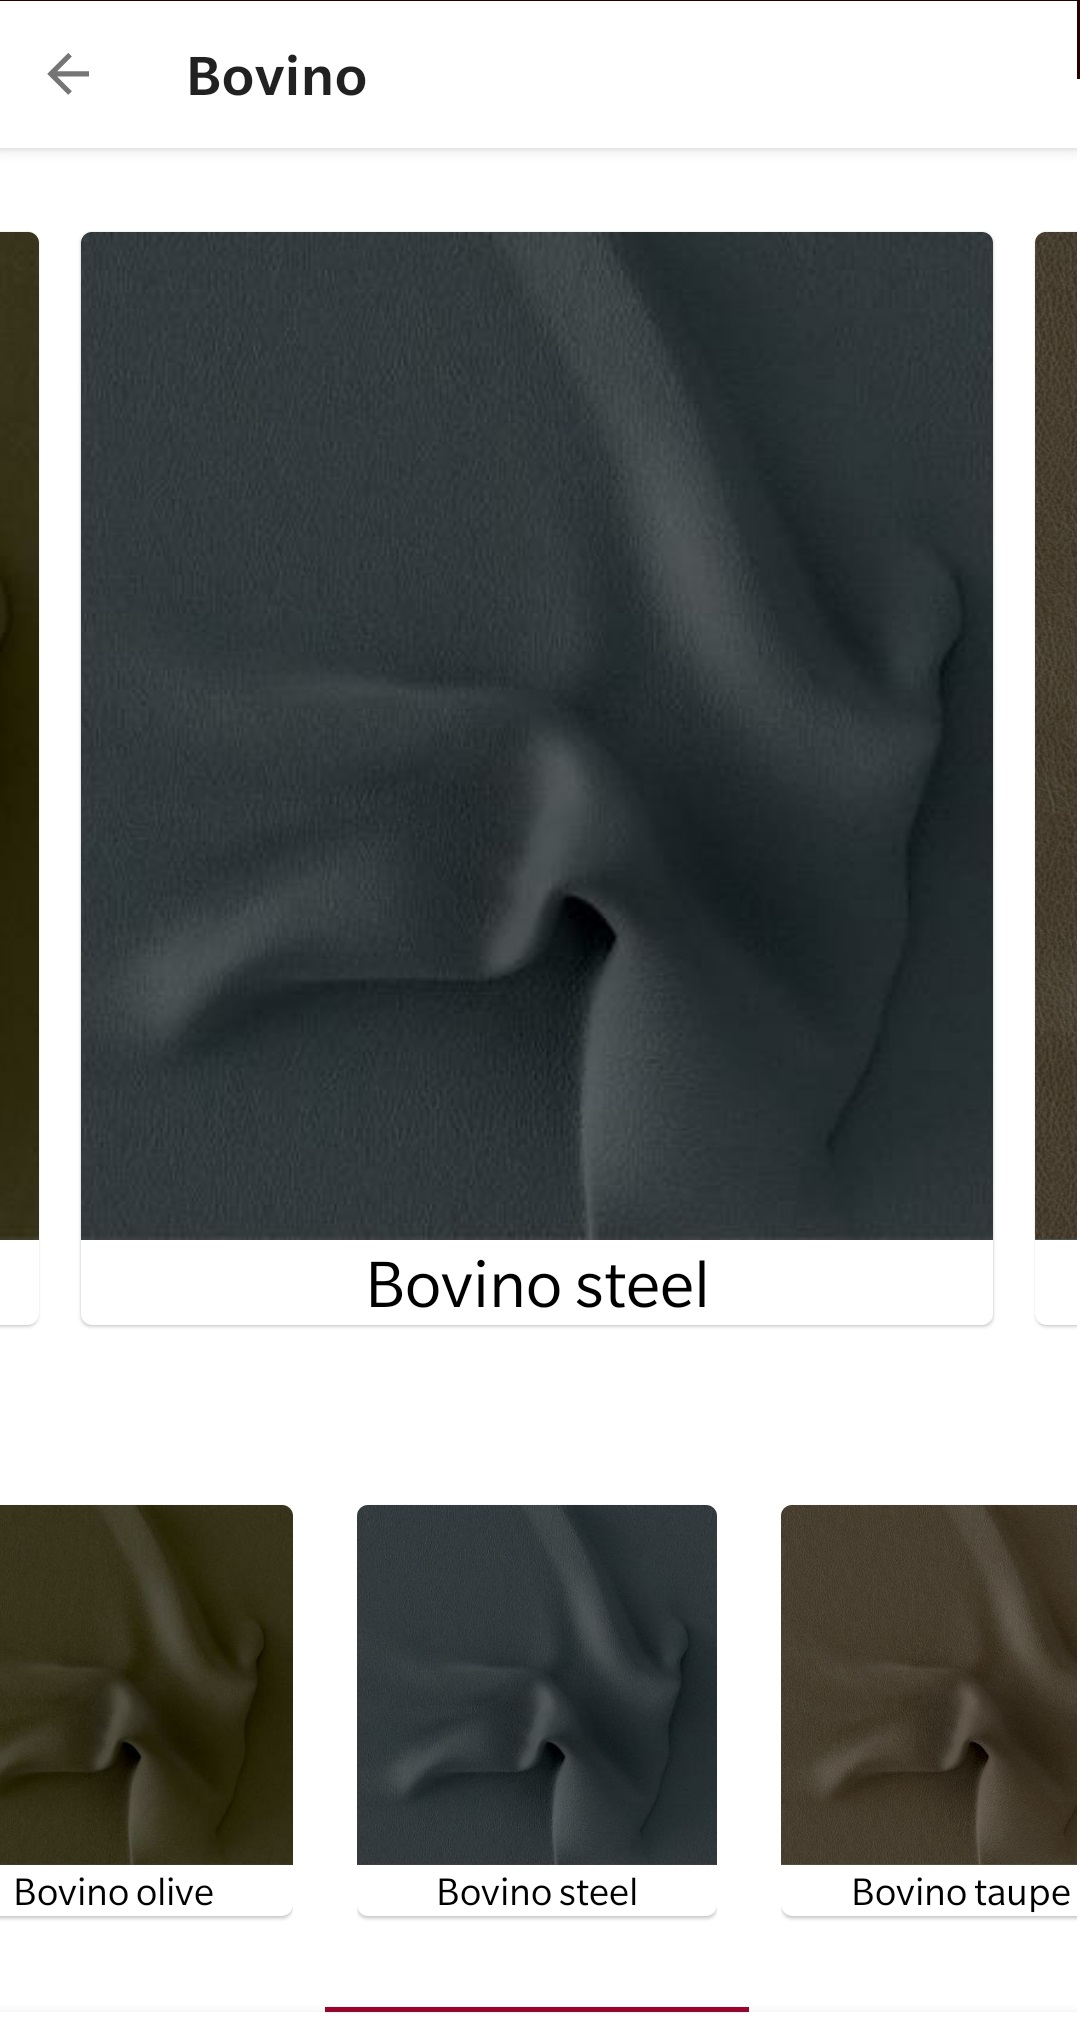
\includegraphics[width=1\textwidth]{img/Screenshot_Cover.jpg}}\\
        \source{eigene Darstellung}
        \label{fig:screenshot_cover_family}
    \end{minipage}
\end{figure}

\FloatBarrier
\subsection{Neuigkeitenseite}
% Termine um auf dem laufenden zu bleiben: Außendienstler
% Schulungen: Möbelhausverkäufer
% Bild für Emotionen (Menschen und Möbel)
% Imagefilm Kundenbindung
% OSGN: für verschiedene Geräte optimiert, im selben Kontext, Firmenzeitschrift
% Banner für verschiedene Größen
% Problem mit zu großer Bitmap
% IT-5384 + IT-5385

Als Letztes wurde die Neuigkeitenseite eingebaut. Die Inhalte dieser Seite wurden von der Marketingabteilung definiert. Dazu gehören Firmenlogo, ein Emotionsbild, anstehende Termine und Messen, Informationen zu Schulungen und eine Verknüpfung zur Firmenwebsite. Die Termine und Schulungen wurden statisch in die Ansicht einprogrammiert. Um sicherzustellen, dass die Bilder auf allen Geräten scharf dargestellt werden, wurde in diesem Fall eine Auflösung von 2000 Pixeln in der Breite gewählt. Dies kann auf leistungsschwächeren Geräten zu einer hohen Arbeitsspeicherauslastung führen. Deswegen wurden die Bilder für alle Geräteklassen, wie in Kapitel \ref{sec:geraeteklassen} erwähnt, skaliert und separat abgelegt.

Die Website öffnet sich im Browser des Systems und verlässt damit die Anwendung. Dies geschieht über einen Intent der ans Android-System gesendet wird. Intents können genutzt werden, um mit dem Android-System, zwischen Activities oder mit anderen Apps zu kommunizieren. In Listing \ref{list:intent_website} wird die Nutzung eines Intents zur Öffnung des Webbrowsers gezeigt. Mit der Methode \texttt{startActivity} in Zeile drei wird der Intent an das Android-System gesendet. Dieses sucht dann die passende Anwendung für die Aufgabe, also den Standardwebbrowser, und übergibt zum Start die \gls{URL} als Argument. Für den Fall, dass kein Browser auf dem Gerät installiert ist, tritt der \texttt{ActivityNotFoundException} Fehler auf. Dieser wird hier abgefangen, um dem Nutzer eine entsprechende Fehlermeldung zu zeigen. Dafür wird ein Android Toast erzeugt. Toasts sind Nachrichten, die am unteren Bildschirmrand temporär angezeigt werden.\footnote{\cite[Vgl.][]{AndroidToasts2019}} Mit der Implementierung der Website sind die letzten User-Stories IT-5384 und IT-5385 abgeschlossen.

\begin{figure}[!htb]
    \centering
    \begin{minipage}[t]{0.6\textwidth}
        \caption{Screenshot der Neuigkeitenseite}
        \frame{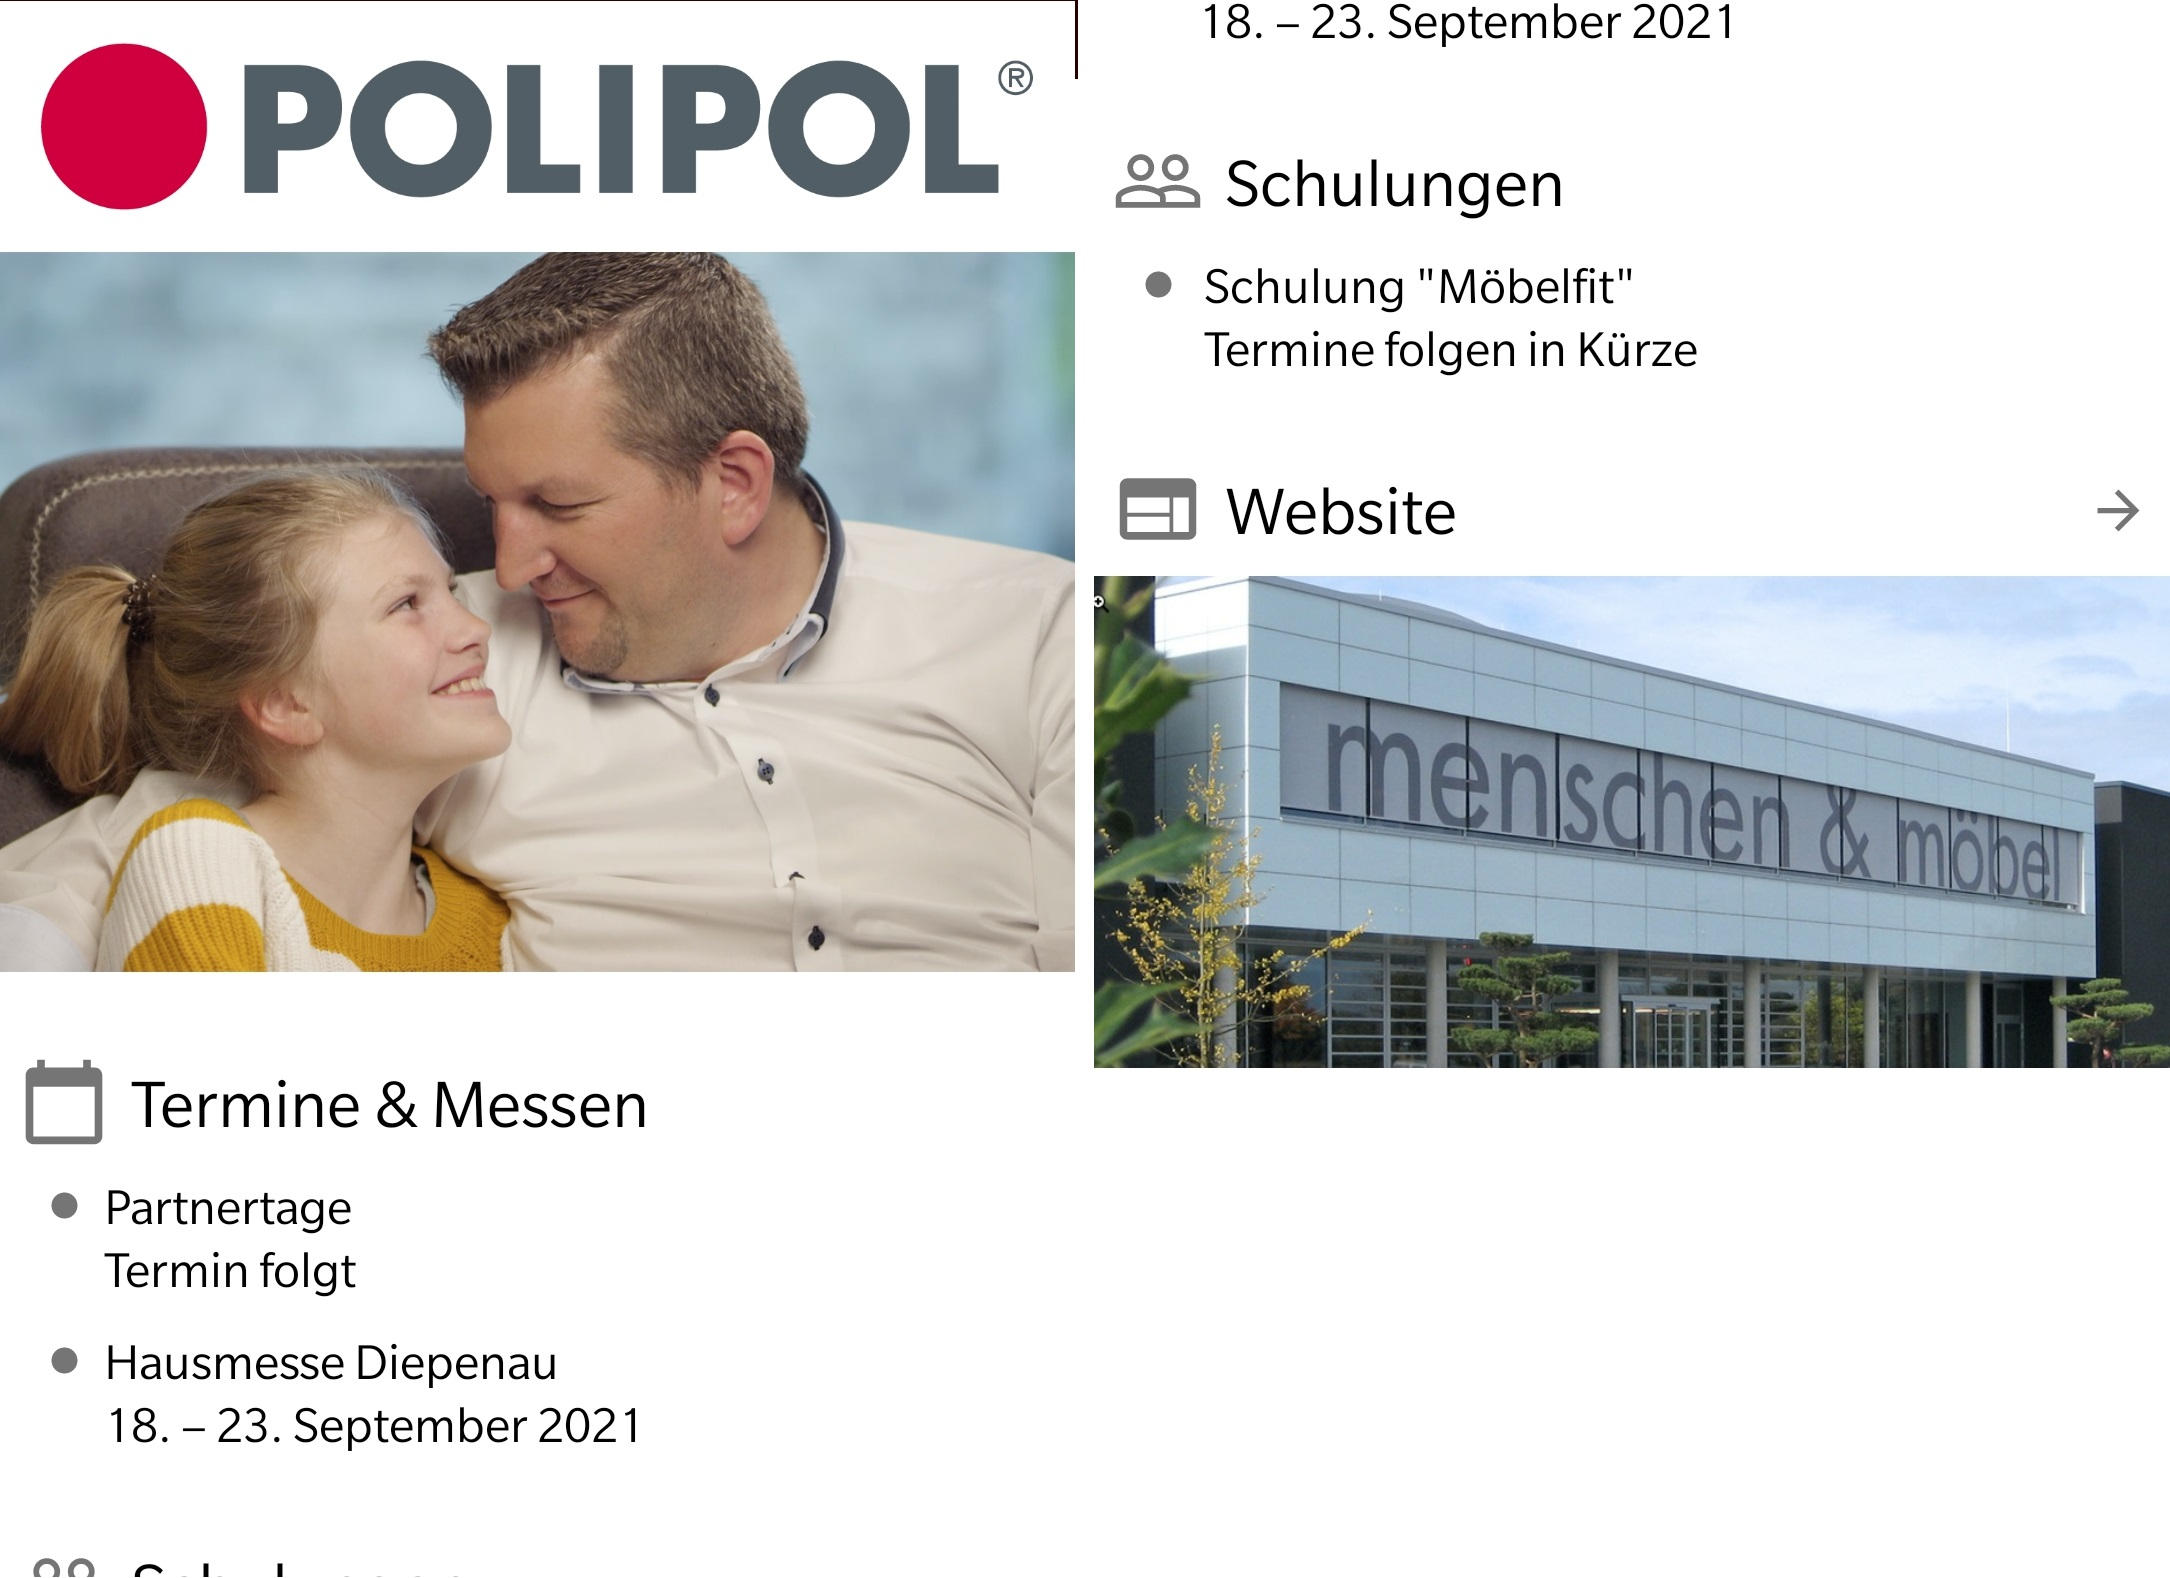
\includegraphics[width=1\textwidth]{img/Screenshot_News.jpg}}\\
        \source{eigene Darstellung}
        \label{fig:screenshot_news}
    \end{minipage}
\end{figure}

\begin{figure}[!htb]
    \begin{lstlisting}[caption=Aufruf des Browsers über das System, label=list:intent_website]
val intent = Intent(Intent.ACTION_VIEW, Uri.parse("https://www.polipol.de")
try {
    startActivity(intent)
} catch (ex: ActivityNotFoundException) {
    val message = context.getString(R.string.error_web_not_available)
    Toast.makeText(context, message, Toast.LENGTH_LONG).show()
}
    \end{lstlisting}
\end{figure}

\clearpage

\section{Feedback}
\label{sec:feedback}
% Positiv:
% Modellfilter durchweg sehr gutes Feedback erhalten. Intuitiv bedienbar (Icons sehr cool)
% Sortimentsübersichtsseite
% Navigation alles direkt gefunden (Informationen zu einem Modell schnell gefunden, Nutzung von Pfeilen, Cards)

% Negativ:
% Galerie (Vollbild, Gesamtübersicht, langes Scrollen)
% Modelldetailseite wirkt etwas überladen
% Zurücksetzen Button im Filter
% Navigation im Typenplan schwer (teilweise noch viel Scrollen, Suchfeld)
% Inhalt (mehr Eigenschaften zu den Stoffen einsehen, eher nichtssagend)

Nach der Fertigstellung des Prototypen konnte bereits erstes internes Feedback gesammelt werden. Getestet wurde durch die Anforderer. Positiv aufgefallen sind vor allem der Modellfilter und die Sortimentsübersichtsseite. Diese zeichneten sich durch eine intuitive Bedienung aus. Die Nutzung von Symbolen in der App wurde im Ganzen ebenfalls positiv bewertet. Dies fiel besonders im Filter und der Modellseite auf. Die Tester hatten keine Probleme die Anwendung zu navigieren. Die Bewertung der Benutzeroberfläche ist überwiegend positiv ausgefallen. Bemängelt wurde hierbei, dass die Modellseite überladen wirkt. Gerade die Galerie war für die meisten Tester schwer zu bedienen. Die Bilder könnten nicht gut überblickt werden. Auch im Typenplan stellte es sich als schwierig heraus, gezielt einzelne Elemente zu finden. Außerdem hatten einige Tester mit der Modellsuche Probleme, da diese keine Toleranz bei Abweichungen bietet. Inhaltlich wünschen sich die Tester mehr Informationen zu den Bezügen und eine Vollbildfunktion für die Galerie Bilder. Technische Probleme traten beim Test nicht auf.

\clearpage